% flatex input: [ICOSSAR_2021_template.tex]
%%%%%%%%%%%%%%%%%%%%%%%%%%%%%%%%%%%%%%%%%%%%%%%%%%%%%%%%%%%%%%%%%%%%%%%%%%%
%%  ICOSSAR2021-Full-paper.tex:   24/09/2020          			         %%
%%  The content, structure, format and layout of this style file is the  %%
%%  property of Research Publishing Services                             %%
%%  Copyright (c) 2020 Research Publishing Services,                     %%
%%  All rights are reserved.                                             %%
%%%%%%%%%%%%%%%%%%%%%%%%%%%%%%%%%%%%%%%%%%%%%%%%%%%%%%%%%%%%%%%%%%%%%%%%%%%

\documentclass[12pt,twocolumn]{article}
\setlength{\columnsep}{7mm}

% All packages needed are put in 'Settings.tex' file
% flatex input: [Settings.tex]
% -------------- Packages
% basic packages and settings - please don't change it
\usepackage{xfrac}
\usepackage{abstract}
\renewcommand{\abstractname}{}    % clear the title
\renewcommand{\absnamepos}{empty} % originally center
\usepackage{float}
\usepackage[utf8]{inputenc}
\usepackage{fontspec}
\usepackage[T1]{fontenc}
\usepackage{mathptmx}
\usepackage[fleqn]{amsmath}
\setlength{\mathindent}{0pt}
\usepackage{geometry}
\geometry{
 a4paper,
 total={160mm,247mm},
 left=25mm,
 right=25mm,
 top=25mm,
 bottom=25mm
}
\usepackage{mwe}
\usepackage{afterpage}

\usepackage{graphicx}
\usepackage[export]{adjustbox}
\usepackage[compatV3]{fancyhdr}
\fancyhf{}

\usepackage{caption}
\captionsetup[table]{skip=-10pt, font=footnotesize, labelformat=simple}
\captionsetup[figure]{skip=10pt,font=footnotesize, labelformat=simple}

\usepackage{enumerate}
\usepackage{hyperref}
\hypersetup{hidelinks}

\usepackage{authblk}
\renewcommand*{\Authfont}{\twelve}
\renewcommand*{\Affilfont}{\nine\it\vspace*{-3pt}}
\setlength{\affilsep}{12pt}

% If no hyphen is allowed
% \usepackage[none]{hyphenat}

\usepackage{color}

% For the header font type
% Arial
\setsansfont[
ItalicFont=ariali.ttf,
]{arial.ttf}

\usepackage{fancyhdr}
% customerized fancyhdr
\pagestyle{fancy}
\setlength{\voffset}{-3mm}
\fancyhead{}
\fancyfoot{}
\fancyhead[L]{
\includegraphics[height=25mm]{figures/IASSAR_Logo.png}}
\fancyhead[R]{

\includegraphics[height=18mm]{figures/ICOSSAR2021_Logo.png}\\
\vspace*{-10pt}
\ten
\color{blue}
{
\sffamily
\textit{
The 13th International Conference on Structural\\
Safety and Reliability (ICOSSAR 2021),\\
June 21-25, 2021, Shanghai, P.R. China\\
J. Li, Pol D. Spanos, J.B. Chen \& Y.B. Peng (Eds)}
}
}
\renewcommand{\headrulewidth}{0pt}
\setlength{\headsep}{0pt}
% \setlength{\headheight}{103.56499pt}
% user required packages or settings


\usepackage{booktabs}
% % \usepackage{capt-of}
% % \usepackage{ragged2e}
%
\usepackage{tabularx}
%
% \usepackage{array}
% \newcolumntype{L}[1]{>{\raggedright\let\newline\\\arraybackslash\hspace{0pt}}m{#1}}
% \newcolumntype{C}[1]{>{\centering\let\newline\\\arraybackslash\hspace{0pt}}m{#1}}
% \newcolumntype{R}[1]{>{\raggedleft\let\newline\\\arraybackslash\hspace{0pt}}m{#1}}
%
% \renewcommand{\arraystretch}{1.3}
% \renewcommand{\floatpagefraction}{1}
% \renewcommand{\textfraction}{0}
% \renewcommand{\dbltopfraction }{1}
% \renewcommand{\topfraction }{1}

% -------------- FontSize --------------
\newcommand{\seven}{\fontsize{7pt}{\baselineskip}\selectfont}    % 7pt
\newcommand{\nine}{\fontsize{9pt}{\baselineskip}\selectfont}    % 9pt
\newcommand{\ten}{\fontsize{10pt}{\baselineskip}\selectfont}    % 10pt
\newcommand{\twelve}{\fontsize{12pt}{\baselineskip}\selectfont} % 12pt
\newcommand{\fourt}{\fontsize{14pt}{\baselineskip}\selectfont}  % 14pt
\newcommand{\sixt}{\fontsize{16pt}{\baselineskip}\selectfont}   % 16pt



\usepackage{titlesec}
% Fontsize of sections
\titleformat{\section}
	{\fontsize{12}{0}\selectfont}{\thesection}{1em}{\normalfont}
% Fontsize of subsections
\titleformat{\subsection}
	{\fontsize{12}{0}\selectfont}{\thesubsection}{1em}{\itshape}
% Fontsize of subsubsections
\titleformat{\subsubsection}
	{\fontsize{12}{0}\selectfont}{\thesubsubsection}{1em}{\itshape}

\usepackage{etoolbox}

\usepackage{academicons}
\usepackage{xcolor}

\newcommand{\orcid}[1]{\href{https://orcid.org/#1}{\textcolor[HTML]{A6CE39}{\aiOrcid}}}

% flatex input end: [Settings.tex]

% All packages needed are put in 'Settings.tex' file

% All packages needed are put in 'Settings.tex' file

\begin{document}

% Font size in tables
\BeforeBeginEnvironment{tabular}{\begin{center}\ten}
\AfterEndEnvironment{tabular}{\end{center}}

% Here put the title name ...
\newcommand{\mytitle}{Tensor Network Contraction For Network Reliability Estimates}

% Please DO NOT change it...
\title{\sixt \bf \vspace*{25mm} \mytitle \vspace*{-20pt}}

% Here put the author name(s)...
\author[a]{Kyle Shepherd \orcid{0000-0002-8220-7448}}
\author[b]{Leonardo Dueñas-Osorio \orcid{0000-0002-7138-7746}}

% Here put the institute name(s) and e-mail(s)...
\affil[a]{PhD Student, Dept. of Civil Engineering, Rice University, Texas, Houston, United States, E-mail: kas20@rice.edu, ORCID:0000-0002-8220-7448}
\affil[b]{Professor, Dept. of Civil Engineering, Rice University, Houston, United States, E-mail: leonardo.duenas-osorio@rice.edu, ORCID:0000-0002-7138-7746}

% Please DO NOT change it...
\pagenumbering{gobble}
% >>>>>>>>>>>>>>>>>>>>>>>>>>>>>>>>>>>>>>>>>>>>>>>>>>>>>
\twocolumn[

\date{}
\maketitle
\thispagestyle{fancy}
\vspace*{-36pt}

% Here start your abstract...
\begin{abstract}
	\noindent

	ABSTRACT: Quantifying network reliability is a hard problem, proven to be \#P-complete \cite{valiant1979complexity}. For real-world network planning and decision making, approximations for the network reliability problem are necessary. This study shows that tensor network contraction (TNC) methods can quickly estimate an upper bound of All Terminal Reliability, $Rel_{ATR}(G)$, by solving a superset of the network reliability problem: the edge cover problem, $EC(G)$. In addition, these tensor contraction methods can exactly solve source-terminal (S-T) reliability for the class of directed acyclic networks, $Rel_{S-T}(G)$.

    The computational complexity of TNC methods is parameterized by treewidth, significantly benefitting from recent advancements in approximate tree decomposition algorithms \cite{dell2018pace}. This parameterization does not rely on the reliability of the graph, which means these tensor contraction methods can determine reliability faster than Monte Carlo methods on highly reliable networks, while also providing exact answers or guaranteed upper bound estimates. These tensor contraction methods are applied to grid graphs, random cubic graphs, and a selection of 58 power transmission networks \cite{li2016characterizing}, demonstrating computational efficiency and effective approximation using $EC(G)$.
    %
    % Most network reliability estimations are performed using randomized methods that output probabilistic bounds, such as direct Monte Carlo simulation (MCS) or fully polynomial randomized approximation schemes (FPRAS) \cite{karger2001randomized}. In contrast, our method exactly bounds the uncertainty of the true value, so as to better inform stakeholders of the worst case scenarios in their critical infrastructure missions.
    %
    % Exact bounds are obtained in this study by solving a superset of the network reliability problem: the edge cover problem. Despite being \#P-complete, many practical solvers exist such as d4 \cite{lagniez2017improved}. However, the topological structures of infrastructure networks can be exploited anew by endowing nodes and links of the networks with tensors, whose logic maps onto the constraints of counting edge covers. The resulting tensor contractions take advantage of the structure of common infrastructure networks and solve many cases that existing competitive solvers cannot solve.
    %
    % We show that our tensor contractions offer computational advantages relative to state-of-the-art methods on problems with manageable treewidth (which can now be efficiently approximated \cite{dell2018pace}), and with favorable topological properties consistent with engineered networks, such as low degree nodes. Our method can also exploit progress on linear algebra and highly optimized matrix operation libraries on CPUs and GPUs, unlike alternatives that rely on conditional operations.
    %
    % In sum, tensor contractions can practically bound network reliability estimates for decision making, and strike a balance between asymptotic errors and guaranteed error estimation for critical infrastructure applications.
\end{abstract}


\vspace*{20pt}
% Please keep this closing bracket to complete the single column format for abstract.
]

% >>>>>>>>>>>>>>>>>>>>>>>>>>>>>>>>>>>>>>>>>>>>>>>>>>>>>

% Here start your contexts...

\BeforeBeginEnvironment{tabularx}{\begin{center}\seven}
\AfterEndEnvironment{tabularx}{\end{center}}

\addtolength{\textfloatsep}{-0.2in}
% flatex input: [manuscript.tex]
\hypertarget{introduction}{%
\section{Introduction}\label{introduction}}

\hypertarget{motivation}{%
\subsection{Motivation}\label{motivation}}

Important infrastructure systems such as electrical transmission grids, potable water distribution, and roadway transportation have been modeled as networks for analysis and design \cite{levy1967monte} \cite{cotilla2012comparing}. As these networks grow in size and become more complex, such as the addition of distributed power generation and energy storage in electrical networks \cite{escalera2018survey}, better algorithms are needed to analyze these networks and guarantee their safety and reliability. The tensor network contraction (TNC) algorithm we propose in this work is a step in this direction.

\hypertarget{problem-definition}{%
\subsection{Problem Definition}\label{problem-definition}}

A network is a graph consisting of nodes that describe a discrete component of the network (such as a power plant or household) and edges that describe a connection between two nodes (such as power lines or water pipes). We will consider a model of a graph \(G = (N,E)\) where \(N\) is the set of labeled nodes \(n_1,...,n_{|N|}\) and \(E\) is the set of labeled edges \(e_1,...,e_{|E|}\). Each node \(n_i \in N\) has a list of attributes \([S,T]\). In particular, \(n_i.S\), the \(S\) attribute of variable \(n_i\), is a Boolean variable equal to \(True\) if \(n_i\) is a source node, and \(n_i.T\) is a Boolean variable equal to \(True\) if \(n_i\) is a terminal node. Each edge \(e_i \in E\) has a list of attributes \([n_p,n_s,bi,p]\). In particular, \(e_i.n_p\) is the predecessor node, \(e_i.n_s\) is the successor node, \(e_i.bi\) is a Boolean variable equal to \(True\) if the edge is bidirectional and \(False\) if the edge is directed, and \(e_i.p\) is the edge reliability, the probability the edge exists.

To measure graph reliability, we define a function \(C(G_r)\), where \(C(G_r)=1\) if there is a path from a source node to every terminal node for the particular graph realization \(G_r\), indicating a Connected graph, and \(C(G_r)=0\) otherwise. A graph realization is defined with a vector \(r\) of length \(|E|\) where \(r_i=1\) if \(e_i\) exists, and \(r_i=0\) otherwise. The probability of a given graph realization is defined below: \[P(G_r) = \prod_{i=1}^{|E|} 1-r_i-e_i.p+2*r_i*e_i.p\] The set of all possible realization vectors is \(R\). This set contains \(2^{|E|}\) elements.

Reliability is defined as \(Rel(G) = \sum_{r \in R} [C(G_r)*P(G_r)]\). \(Rel(G)\) will take on a value between 0 and 1, where a higher \(Rel(G)\) is desired in practice.

This model as defined allows us to consider two cases of network reliability that are important for managers of infrastructure systems. All Terminal Reliability is \(Rel_{ATR}(G)\) where all edges are bidirectional and all nodes are terminal nodes. Source-Terminal reliability is \(Rel_{S-T}(G)\) where all edges are directed, and in general the set of source and terminal nodes is much smaller than the set of nodes. For this work, only one source and one terminal node will be considered for \(Rel_{S-T}(G)\) (also known as 2-terminal reliability).

\hypertarget{justification-and-objectives}{%
\subsection{Justification and Objectives}\label{justification-and-objectives}}

As the time to compute the reliability of a probabilistic graph scales exponentially with the size of the graph \cite{valiant1979complexity}, a naïve brute force enumeration of all graph realizations is not feasible for the large graphs frequently encountered in infrastructure systems. Therefore, different approaches are needed to calculate values of \(Rel(G)\).

One approach is to develop an algorithm with parameterized complexity to solve \(Rel(G)\). While these algorithms may scale exponentially in the worst case, they may not scale as fast for the problems we are interested in. Another approach is to solve a superset problem of \(Rel(G)\). In this work, the edge cover problem will be shown to be a superset problem of \(Rel_{ATR}(G)\). A final approach is to give up on obtaining an exact answer and instead obtain an approximate answer for \(Rel(G)\) using Monte Carlo (MC) simulation.

The objective of this work is to efficiently calculate values of \(Rel(G)\) in a principled way. This work will formulate TNC algorithms for exactly solving \(Rel_{S-T}(G)\) when the graph is directed and acyclic, and exactly solving an upper bound for \(Rel_{ATR}(G)\) by solving the edge cover problem. These proposed TNC algorithms will be shown to have computational complexity parameterized by the treewidth of the graph. The performance of these algorithms will be tested on grid graphs, random cubic graphs, and a selection of real world transmission graphs.

\hypertarget{background}{%
\section{Background}\label{background}}

\hypertarget{exact-solvers}{%
\subsection{Exact Solvers}\label{exact-solvers}}

\hypertarget{binary-decision-diagram-methods}{%
\paragraph{\texorpdfstring{Binary Decision Diagram Methods\\
}{Binary Decision Diagram Methods }}\label{binary-decision-diagram-methods}}

The current state-of-the-art for exactly solving undirected K-Terminal reliability problems (which includes ATR and S-T) is using binary decision diagrams \cite{carlier1996decomposition}. These methods consider one edge at a time, factoring the graph into subgraphs, and pruning by identifying isomorphic graphs \cite{hardy2007k}.

However, the pruning is not very efficient. In the worst case for All Terminal Reliability problems, the number of subgraphs to be considered is proportional to \(BELL(F_{max})\), where \(BELL(k)\) is the \(k^{th}\) bell number and \(F_{max}\) is the linear-width, or pathwidth, of the graph. If the pathwidth of the graph is small, this algorithm is still useful, but \(BELL(k)>(\frac{k}{e\ln(k)})^k\) \cite{berend2010improved}, growing faster than \(2^n\), so binary decision diagram methods quickly become computationally infeasible.

\hypertarget{sat-solvers}{%
\paragraph{\texorpdfstring{\#SAT solvers\\
}{\#SAT solvers }}\label{sat-solvers}}

The edge cover problem \(Rel_{EC}(G)\) is a superset of \(Rel_{ATR}(G)\). We can define \[Rel_{EC}(G) = \sum_{r \in R} [EC(G_r)*P(G_r)]\] where \(EC(G_r)=1\) if every node has at least one existing edge, and \(EC(G_r)=0\) otherwise. \(Rel_{ATR}(G) \subset Rel_{EC}(G)\) because for every case of \(Rel_{ATR}(G)\) every node must have at least one existing edge to ensure connectivity, but \(Rel_{EC}(G) \not\subset Rel_{ATR}(G)\) because unconnected ``islands'' of nodes can satisfy \(EC(G_r)\) while not satisfying global connectivity for \(C(G_r)\).

Rewritten in conjunctive normal form (CNF) as a monotone \#SAT problem \cite{roth1996hardness} \cite{vaisman2015model}: \[EC(G_r) = \bigwedge_{n_i \in N} (\bigvee_{j \in n_i} e_j(r))\] where each node \(n\) has a set of associated edges \(j \in n_i\) if edge \(e_j\) has node \(n_i\) as a predecessor or successor. The function \(e_j(r)\) is equal to True if \(r_j=1\) for graph realization \(r\).

Our ability to write this problem in CNF form, a set of clauses which all must be true, and each clause is satisfied if at least one variable in the clause is true, allows it to be solved by powerful existing model counting solvers such as cachet \cite{sang2005heuristics}, miniC2D \cite{oztok2015top}, and d4 \cite{lagniez2017improved}. However, these solvers are considered to be ``black-box'' solvers, so there is no ability to estimate their computation time for an arbitrary graph \(G\).

\hypertarget{probabilistic-solvers}{%
\subsection{Probabilistic Solvers}\label{probabilistic-solvers}}

\hypertarget{monte-carlo-mc-methods}{%
\paragraph{\texorpdfstring{Monte Carlo (MC) Methods\\
}{Monte Carlo (MC) Methods }}\label{monte-carlo-mc-methods}}

If a set of \(K\) independent random realizations of a given graph are generated, \(G_{rand}\), then \(Rel(G)\) can be estimated from this random sample of graphs. \(C(G_{rand})\) can be considered to be a set of Bernoulli trials, a binomial experiment \(B(K,p)\) so MC methods can be used to estimate the \(p\) of the Bernoulli process and provide a confidence interval.

Given a specific simulation of \(G_{rand}\), the log-likelihood profile of \(p\) can be obtained. The most likely value of \(p\), \(p_{true}\), is obtained by finding the maximum of the profile. To obtain a confidence interval, we can use the profile likelihood method \cite{venzon1988method}. For a given desired \(1-\alpha\) and \(\epsilon=\frac{p_{true}}{p_{-(1-\alpha)\%}}\), the number of needed samples \(K\) can be calculated.

For a range of \(\epsilon\) values, Figure \ref{fig:MC Trial Graph} shows on a log-log scale how the number of needed MC samples decreases as \(p_{true}\) increases. Specifically, if \(p_{true}\) increases by a factor of 10, the number of trials needed decreases by a factor of 10 while \(p_{true}<0.1\).

\begin{figure}[t]
\caption{Needed MC trials for a given $\epsilon$ at a 95\% confidence interval shown on a log-log scale graph: As $p_{true}$ decreases, the number of needed MC trials for a given relative error increases.}
\label{fig:MC Trial Graph}
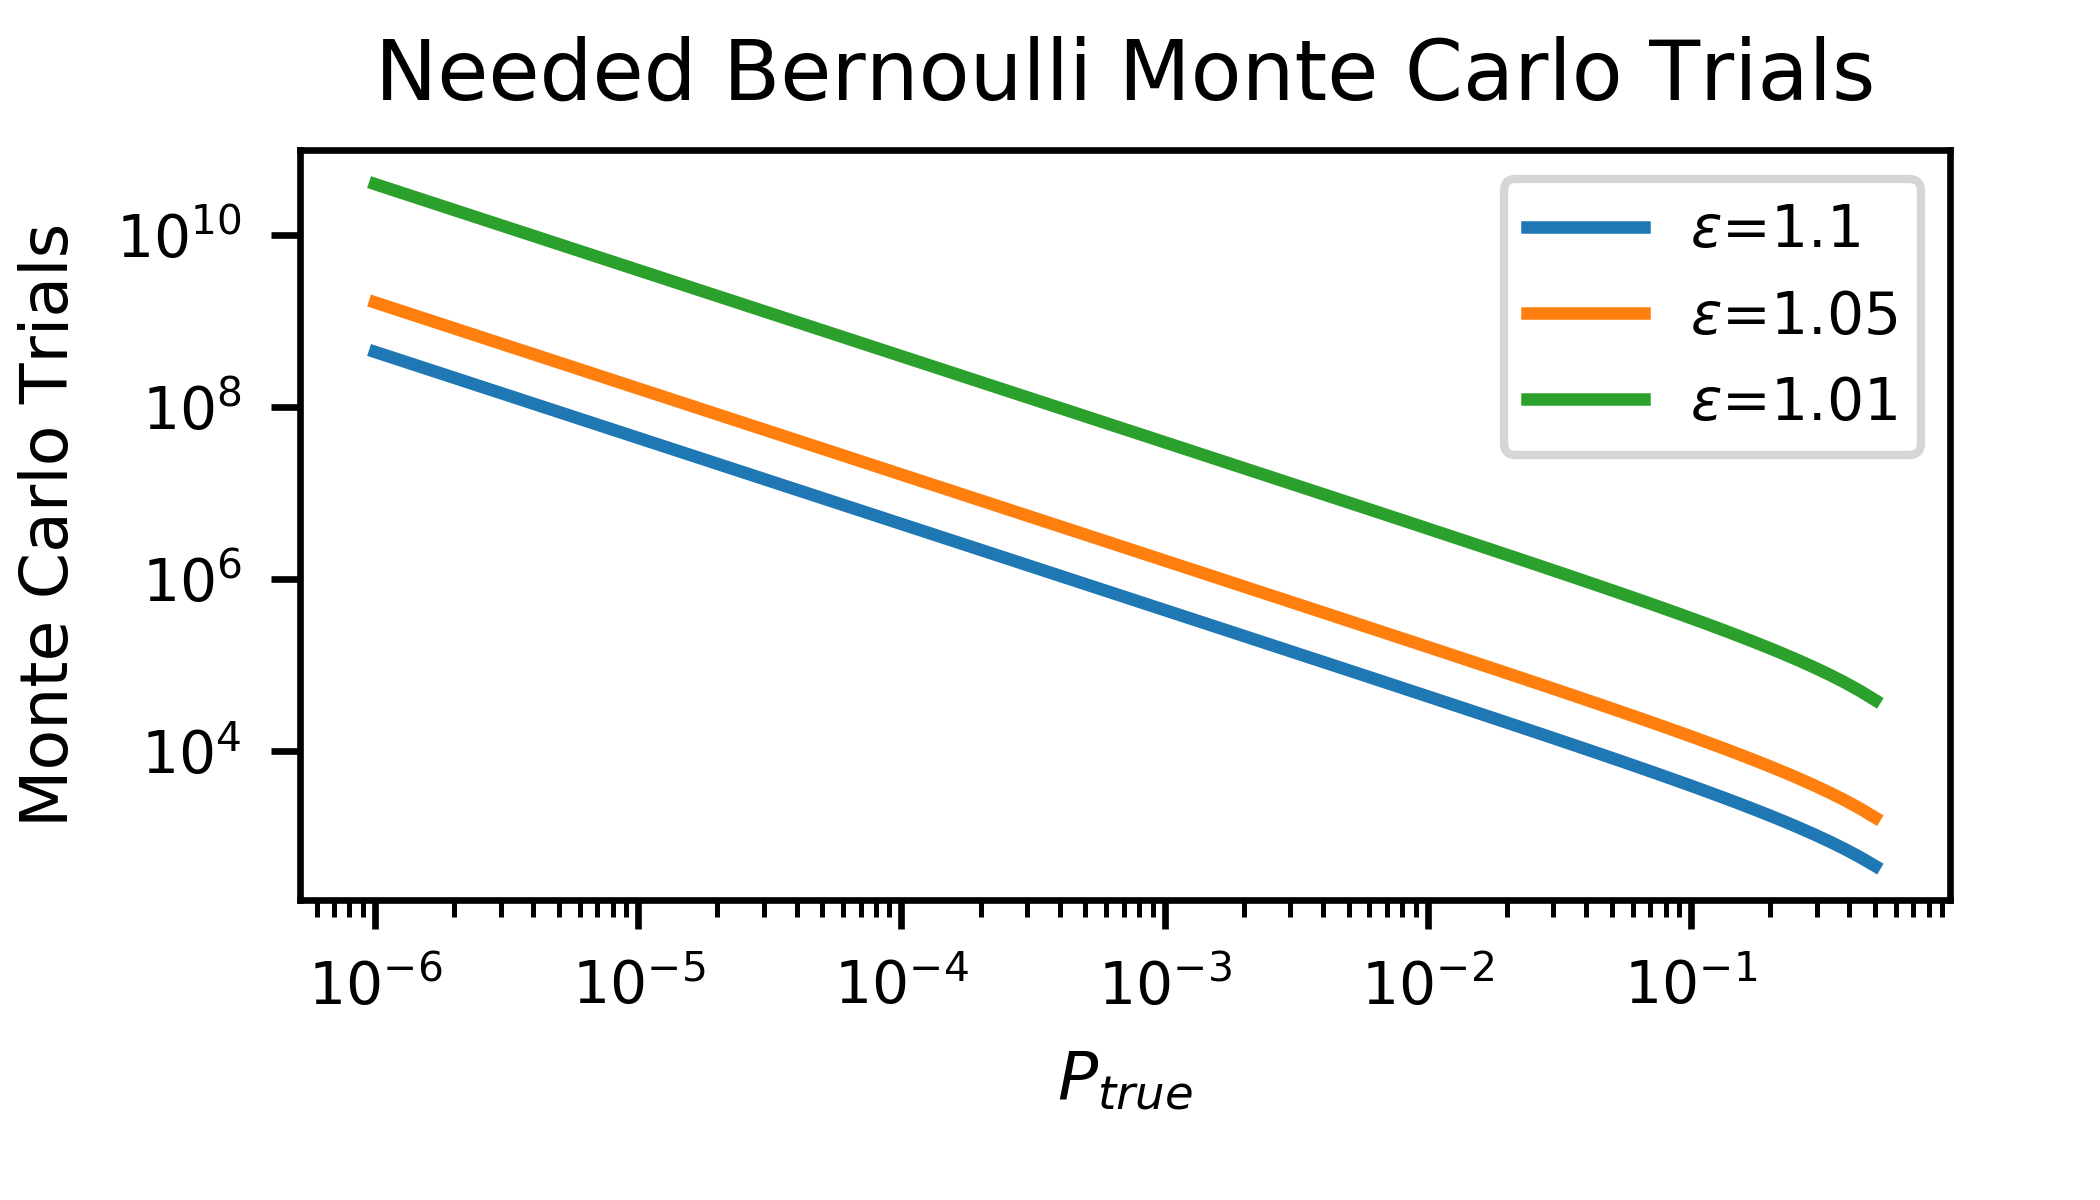
\includegraphics[width=0.5\textwidth]{../figures/MCTrials.png}
\end{figure}

The advantage of MC Methods is the number of samples required is only proportional to \(\frac{1}{p_{true}}\) and is not proportional to the problem size. The drawback is that \(p_{true}\) is not known ahead of time, so the number of samples required could be large if \(p_{true}\) is very small and cannot be known ahead of time, and stopping rules must be used, adding uncertainty.

\hypertarget{fully-polynomial-time-randomized-approximation-scheme-fpras}{%
\paragraph{\texorpdfstring{Fully Polynomial-time Randomized Approximation Scheme (FPRAS)\\
}{Fully Polynomial-time Randomized Approximation Scheme (FPRAS) }}\label{fully-polynomial-time-randomized-approximation-scheme-fpras}}

From the analysis above, MC methods become infeasible for estimating graph failure rates when \(Rel(G)\) is close to 1. In response to this drawback, Karger \cite{karger2001randomized} developed a Fully Polynomial-time Randomized Approximation Scheme (FPRAS) for estimating \((1-Rel_{ATR}(G))\) that runs in \(O(\frac{|E||N|^4}{\epsilon^3}\ln(|N|))\) time.

However, the FPRAS algorithm only works when \((1-Rel_{ATR}(G))<|N|^{-4}\). For most engineering applications, the failure chances we care about are small. For example, 1\% for 50 year earthquake hazards \cite{IBC_2017} or \(2.0*10^{-6}\) per year for nuclear power plants \cite{NRC_2010}. Therefore, highly reliable engineering networks with more than \((1-2.0*10^{-6})^{-\frac{1}{4}} \approx 27\) nodes cannot be practically solved using known FPRAS methods. In addition, this FPRAS algorithm is limited and only works for All-Terminal Reliability. While extensions exist for K-Terminal problems, such as the one developed by Paredes \cite{paredes2019principled} which works well in practical settings, these extensions rely on NP-oracles and therefore have exponential worst case behavior.

Therefore, we desire an approximation algorithm that is not dependent on \(Rel(G)\), and is instead parameterized by some other graph property that is small for engineering networks of interest. TNC algorithms fit this desire, being parameterized by the treewidth of a graph, which is usually small and constrained for the almost-planar engineering networks we care about.

\hypertarget{tensor-network-contraction-tnc}{%
\section{Tensor Network Contraction (TNC)}\label{tensor-network-contraction-tnc}}

\hypertarget{definitions}{%
\subsection{Definitions}\label{definitions}}

The goal of TNC is to write the underlying satisfiability problem as a series of tensor products. Similar techniques have been investigated in the physics community to solve specific quantum mechanics problems \cite{pan2020contracting} \cite{biamonte2019lectures}. Each clause in the satisfiability problem is represented as a tensor \(T^c_{x_1,x_2,...,x_k}\). If the variables \(x_1,x_2,...,x_k\) satisfy the underlying clause, then \(T_{x_1,x_2,...,x_k}=1\). For example, the \(T^c\) that encodes the Boolean clause \((x_1 \lor x_2 \lor x_3 \lor x_4)\) is: \begin{equation*}
T^c_{x_1,x_2,x_3,x_4}=
\begin{cases}
  0, & \text{if}\ x_1=x_2=x_3=x_4=0 \\
  1, & \text{otherwise}
\end{cases}
\end{equation*}

The number of solutions to the satisfiability problem can be calculated by applying the tensor product to every clause tensor \(T^c\). The tensor product is defined as \ten \[T^p_{x_1,...,x_k,z_1,...,z_k}=T^c_{x_1,...,x_k,y_1,...,y_k} \otimes T^c_{y_1,...,y_k,z_1,...,z_k}\] \normalsize where \(\otimes\) expands into \ten \[T^p_{x_1,...,x_k,z_1,...,z_k}=\sum_{y_i \in Y} \sum_{y_i=0}^{|y_i|} T^c_{x_1,...,x_k,y_1,...,y_k} * T^c_{y_1,...,y_k,z_1,...,z_k}\] \normalsize where \(Y\) is the set of all variables in common between the two tensors, and \(|y_i|\) is the number of states that variable \(y_i\) can take. While \(y_i\) can take an arbitrary number of states, the remainder of this work will only consider a two-state Boolean variable.

One complication is that a tensor product is only clearly defined if each variable appears exactly once or twice, while in many satisfiability problems a variable can appear more than twice. This complication can be addressed by assigning each \(T^c\) a unique set of variables, and then creating additional variable tensors \(T^v\) to apply constraints on the variables.

Two common constraints are defined below. To constrain a Boolean variable \(x_1\) to take the opposite value of \(x_2\) (as needed for a Boolean formula containing \(x_1\) and \(\neg x_1\)), the following tensor \(T^v_{x_1,x_2}\) is set as \begin{equation*}
T^v_{x_1,x_2}=
\begin{cases}
  1, & \text{if}\ x_1=0\ \text{and}\ x_2=1\\
  1, & \text{if}\ x_1=1\ \text{and}\ x_2=0\\
  0, & \text{otherwise}
\end{cases}
\end{equation*}

To constrain a Boolean variable \(x_1\) to take the same value of \(x_2\) and apply a probability \(p\) of both variables being true (as needed to define an unreliable network edge), the tensor \(T^v_{x_1,x_2}\) is set as \begin{equation*}
T^v_{x_1,x_2}=
\begin{cases}
    p, & \text{if}\ x_1=1\ \text{and}\ x_2=1 \\
    1-p, & \text{if}\ x_1=0\ \text{and}\ x_2=0 \\
    0, & \text{otherwise}
\end{cases}
\end{equation*}

\hypertarget{graph-representation}{%
\subsection{Graph Representation}\label{graph-representation}}

Tensor multiplications can be represented as a node and edge graph, \(G_T\), where each tensor is a node and each variable is an edge. An example of a tensor graph can be seen in Figure \ref{fig:Tensor Graph Example}a. A tensor product can be represented as an edge contraction on this graph. The contraction of edge \(X_1\) is visually shown in Figure \ref{fig:Tensor Graph Example}b. Once all edges are contacted, only a scalar value remains, counting the number of solutions to the Boolean problem.

\begin{figure}[t]
\caption{Example Tensor Graph [a] and example tensor contraction of edge $X_1$ [b]}
\label{fig:Tensor Graph Example}
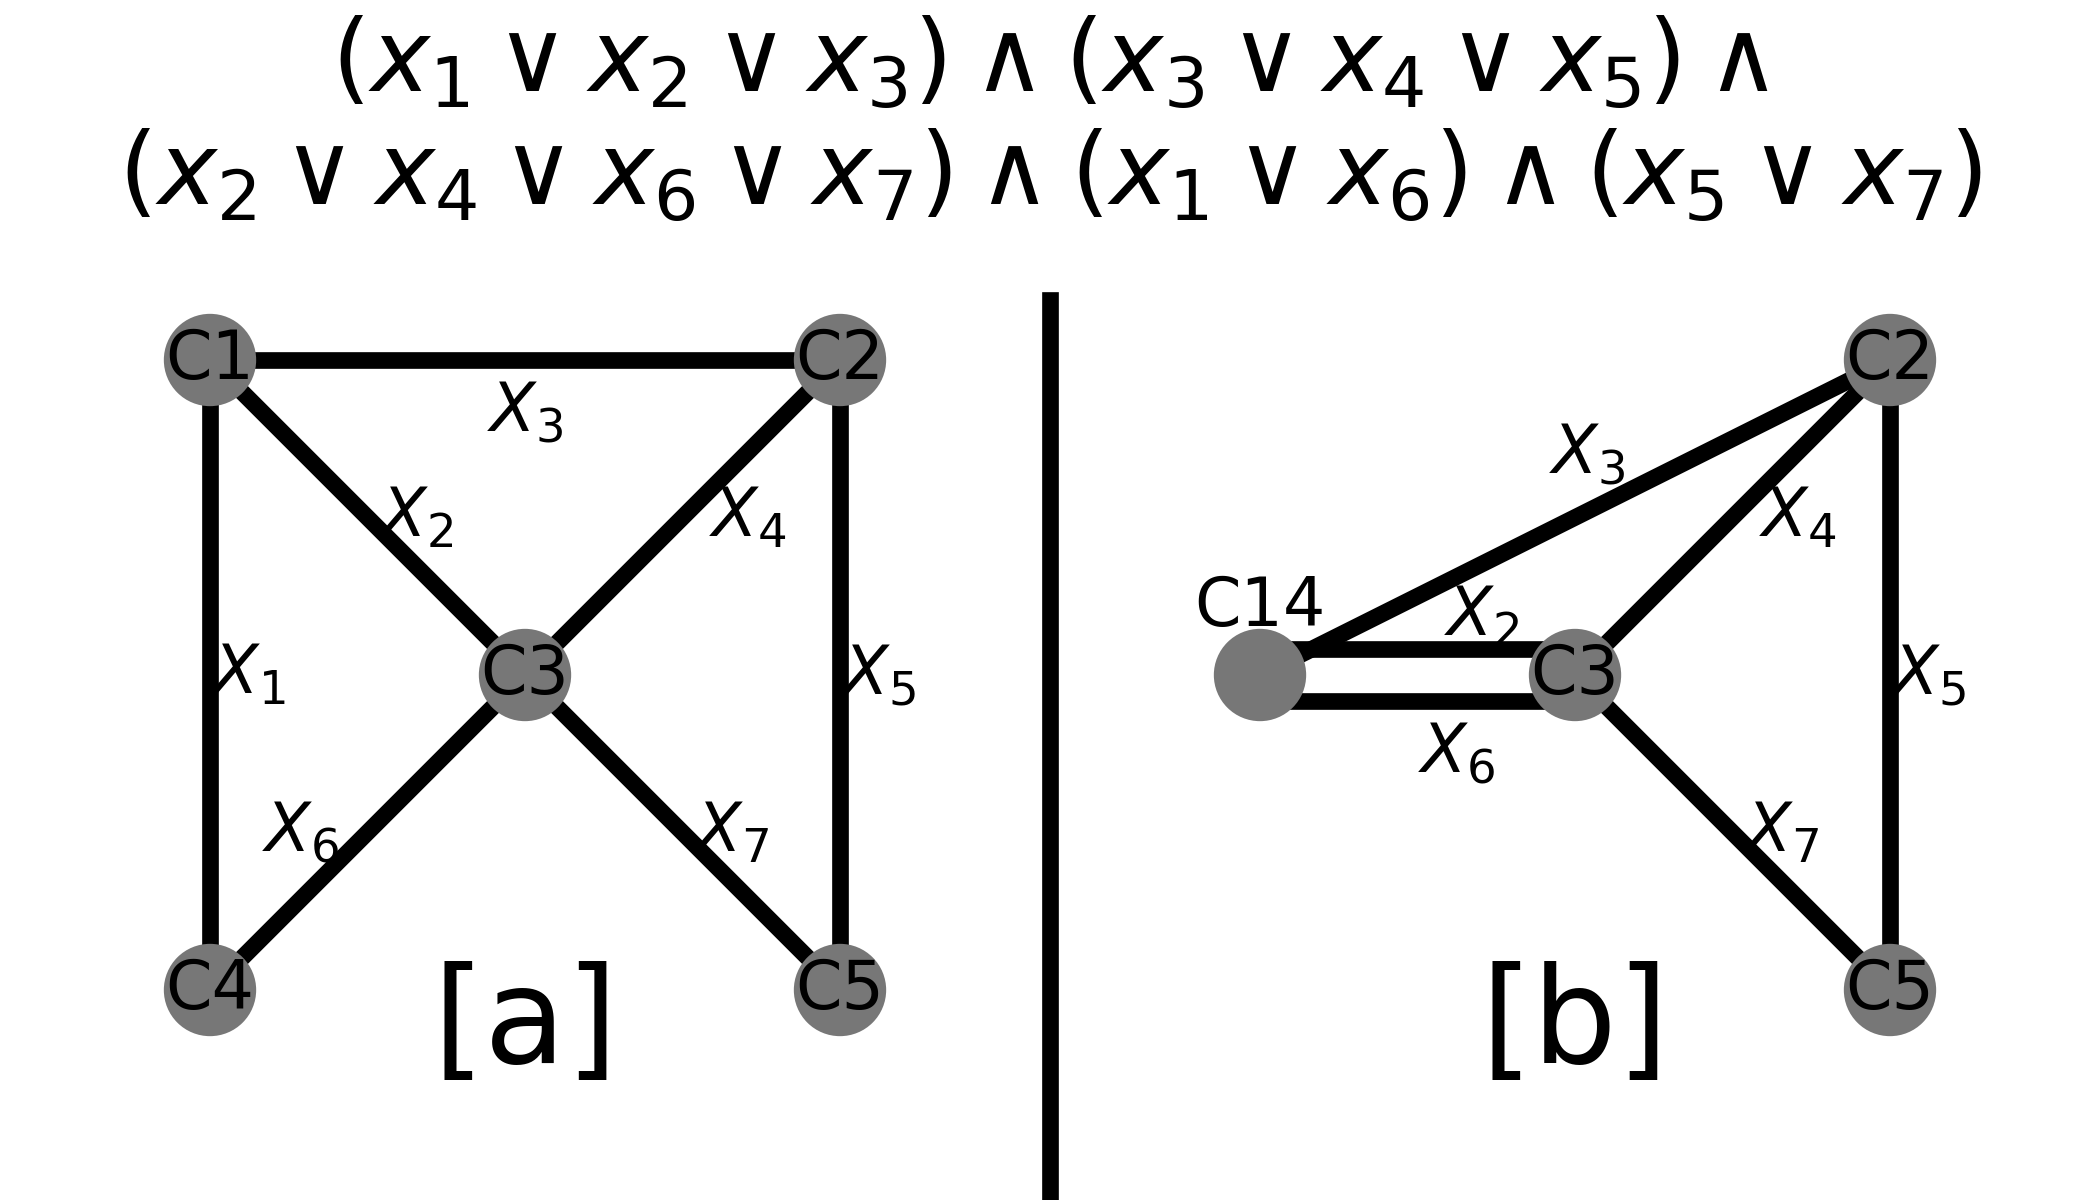
\includegraphics[width=0.5\textwidth]{../figures/TensorGraphExample.png}
\end{figure}

\hypertarget{contraction-ordering}{%
\subsection{Contraction Ordering}\label{contraction-ordering}}

Care must be taken when choosing the order to perform the edge contractions. Assuming Boolean variables, the product \(T^c_{x_1,...,x_n,y_1,...,y_n} \otimes T^c_{y_1,...,y_n,z_1,...,z_n}\) requires \(2^{|x|+|y|+|z|}\) multiplications and additions, and \(2^{|x|+|z|}\) numbers need to be stored in memory for the resulting tensor. Markov, Igor L and Shi, Yaoyun show how to determine an optimal edge contraction ordering to minimize \(|x|\), \(|y|\), and \(|z|\), also known as elimination ordering, from an optimal tree decomposition of the line graph of \(G_T\), \(LG(G_T)\) \cite{markov2008simulating}. Dumitrescu et al.~\cite{dumitrescu2018benchmarking} demonstrate how algorithms from the PACE 2017 challenge \cite{dell2018pace} can be used to obtain better approximate tree decompositions for some tensor graphs representing quantum many body problems.

Harvey, Daniel J and Wood, David R provide a few different upper bounds for the treewidth of \(LG(G_T)\), \(tw(LG(G_T))\), bounding the size of the largest tensor \cite{harvey2018treewidth}: \begin{equation*}
tw(LG(G_T))<(tw(G_T)+1)*D_m(G_T)-1
\end{equation*} where \(D_m(G_T)\) is the maximum degree of graph \(G_T\). Dudek et al.~\cite{dudek2019efficient} also show how high-rank tensors can be factored into a tensor tree to further minimize memory and computational requirements of the TNC.

Overall, in the worst case for infrastructure networks with bounded max degree (due to physical limitations), the largest number of variables for a single tensor is linearly proportional to the treewidth of \(G_T\). Therefore, the computational complexity is at most \(2^{C*tw(G)}\), where C is a constant between 1 and \(D_m(G_T)\).

For the following formulations, if every variable tensor is contracted into an adjacent clause tensor, the resulting tensor graph is isomorphic to the underlying graph \(G\). Therefore, for these formulations, \(tw(G_T)\) is equal to \(tw(G)\).

\hypertarget{all-terminal-reliability-formulation}{%
\subsection{All Terminal Reliability Formulation}\label{all-terminal-reliability-formulation}}

For \(Rel_{ATR}(G)\) there is no known polynomial sized satisfiability equation, unless auxiliary variables are used \cite{paredes2019principled}. Therefore, a tensor graph for the edge cover problem, \(Rel_{EC}(G)\) will be formulated instead. The edge cover problem is satisfied if every node in the graph \(G\) has at least one existing edge. Therefore, the clause for a node \(n\) with connecting edges \(e \in E\) is \((e_1^n \lor e_2^n \lor ... \lor e_i^n)\).

Each edge \(e_i\) has a probability \(p\) of existing, and each variable \(e_i^n\) takes the same correlated state for every superscript \(n\). Contracting the tensor graph \(G_T\) of these tensors will yield the probability of a satisfying edge cover for the graph \(G\).

\hypertarget{s-t-reliability-formulation}{%
\subsection{S-T Reliability Formulation}\label{s-t-reliability-formulation}}

For \(Rel_{S-T}(G)\), the problem is satisfied if any inbound edge connected to the terminal node \(n_t\) is connected to a ``marked'' node. A node is marked if any of its inbound edges is connected to a ``marked'' node or a ``source'' node. For an acyclic directed network, a node \(n_b\) is ``marked'' if and only if there is a path from the source node to node \(n_b\) (This statement does not hold true for graphs with cycles). Even in this restricted case, \(Rel_{S-T}(G)\) is still a \#P-complete problem \cite{provan1986complexity}.

The clause for the terminal node \(n_t\) with inbound edges \(e \in E\) is \((e_1^{n_t} \lor e_2^{n_t} \lor ... \lor e_i^{n_t})\).

For a node between the source and terminal nodes \(n_b\) with inbound edges \(e \in E\), it must satisfy the following clause: \begin{equation*}
\begin{split}
& (m_{n_b} \land (e_1^{n_b} \lor ... \lor e_i^{n_b})) \lor \\
& (\neg m_{n_b} \land \neg (e_1^{n_b} \lor ... \lor e_i^{n_b}))
\end{split}
\end{equation*} where \(m_{n_b}\) is a variable indicating if node \(n_b\) is marked.

For each variable \(e_i\), it must be constrained to only be True with probability \(e_i.p\) when the tail is connected to a ``marked'' or source node, \(m_{n_b}=1\), and always False when the tail is not connected to a ``marked'' node. Therefore, the corresponding variable tensor for edge \(i\) outbound from node \(b\) and inbound to node \(y\) is: \begin{equation*}
\begin{split}
& T^{v_e}_{m_{n_{b,y}},e_i^{n_y}}= \\
& \begin{cases}
  e_i.p, & \text{if}\ m_{n_{b,y}}=1\ \text{and}\ e_i^{n_y}=1 \\
  1-e_i.p, & \text{if}\ m_{n_{b,y}}=1\ \text{and}\ e_i^{n_y}=0 \\
  1, & \text{if}\ m_{n_{b,y}}=0\ \text{and}\ e_i^{n_y}=0 \\
  0, & \text{if}\ m_{n_{b,y}}=0\ \text{and}\ e_i^{n_y}=1 \\
\end{cases}
\end{split}
\end{equation*}

In addition, the directed ``marked'' variable \(m_{n_{b,y}}\) must be constrained to the same value as \(m_{n_b}\). Contracting the tensor graph \(G_T\) of these tensors will yield the exact probability of a satisfying path from the source node to the terminal node for the graph \(G\).

\hypertarget{tensor-network-contraction-tnc-advantages}{%
\subsection{Tensor Network Contraction (TNC) Advantages}\label{tensor-network-contraction-tnc-advantages}}

TNC algorithms have many advantages over the previously described exact solvers and probabilistic solvers. The upper bound computational complexity of \(2^{C*tw(G)}\) is significantly better than the \(BELL(Pathwidth(G))\) of the binary decision diagram methods and the unknown upper bounds of the \#SAT methods. This bound is not dependent on \(Rel(G)\), so TNCs can solve some highly reliable networks faster than probabilistic solvers. The computational effort of a TNC can be known ahead of time (after the approximate tree decomposition), so reliability engineers can confidently choose the most efficient reliability solver algorithm. In addition, for infrastructure networks of interest, they are usually near-planar, which bounds treewidth to \(2*\sqrt{6*(k+1)*|N|})\) \cite{dujmovic2017structure} where k is the number of allowed crossings for each edge, and treewidth is frequently lower than this bound \cite{maniu2019experimental}.

TNCs only require vectorized multiplication and addition operations which are very efficient for CPUs and GPUs to compute, while binary decision diagram methods and \#SAT methods require many conditional if-then statements which are more difficult to optimize. While probabilistic solvers are perfectly parallel (each sample can be done on a separate computer), the individual tensor contractions can also be broken up and dispatched to multiple parallel computing units.

\hypertarget{results-and-discussion}{%
\section{Results and Discussion}\label{results-and-discussion}}

\hypertarget{benchmark-graphs}{%
\subsection{Benchmark Graphs}\label{benchmark-graphs}}

To evaluate the empirical performance of the proposed TNC algorithm, a few classes of graphs will be considered. The first considered class of graphs are grid graphs. As most infrastructure networks are usually near-planar, grid graphs can be considered as the ideal case of planar graphs.

Second, random connected cubic graphs will be considered. Using a set of reliability preserving transformations \cite{shooman1991exact}, and by splitting high degree nodes into a chain of degree 3 nodes connected by unfailing edges, all graphs can be converted to a cubic graph with equivalent \(Rel(G)\). A 1-Flipper Markov Chain Monte Carlo (MCMC) algorithm will be used to uniformly generate these random cubic graphs \cite{feder2006local}.

Third, a collection of 58 US power transmission networks \cite{li2016characterizing} will be considered. These graphs will be reduced using reliability preserving transformations before reliability calculations are performed.

All benchmarks are performed on a Intel Core i7-4810MQ CPU @ 2.90GHz, with 16 GB of RAM. All code is single threaded. The code used to generate these graphs can be seen at this link {[}LINK GITHUB HERE{]}.

\hypertarget{grid-graphs}{%
\subsection{Grid Graphs}\label{grid-graphs}}

\hypertarget{computational-time}{%
\subsubsection{Computational Time}\label{computational-time}}

As seen in Figure \ref{fig:Grid Graph Computational Time}a, as the grid dimension increases, both the number of subgraphs for the binary decision diagram method and the number of floating point operations for the TNC increases exponentially. Figure \ref{fig:Grid Graph Computational Time}b shows the wall clock time taken for each method. In both cases, the slope of the TNC is significantly smaller than the binary decision diagram method, showing significant computational advantages for calculating \(EC(G)\) and \(Rel_{S-T}(G)\).

Further computational advantages can be seen if one dimension of the grid graph is fixed in size (8 nodes is large enough for a non-trivial treewidth size and small enough to be computed quickly by both methods). As seen in Figure \ref{fig:Grid Graph Computational Time}c, as \(n\) increases for the \(8xn\) grids, both the number of subgraphs for the binary decision diagram method and the number of floating point operations for the TNC increases linearly. However, as seen in Figure \ref{fig:Grid Graph Computational Time}d, the wall clock time taken for the binary decision diagram method increases quadratically (each subgraph needs an \(O(|E|)\) connectivity check) while the TNC time only increases linearly. For graphs of bounded treewidth, TNCs show significant computational improvement.

\begin{figure}[t]
\caption{Computational complexity and wall clock time for $nxn$ and $8xn$ grid graphs. Subgraphs and $REL_{ATR}(G)$ are BDD calculations, and floating point operations and $EC(G)$ are TNC calculations.}
\label{fig:Grid Graph Computational Time}
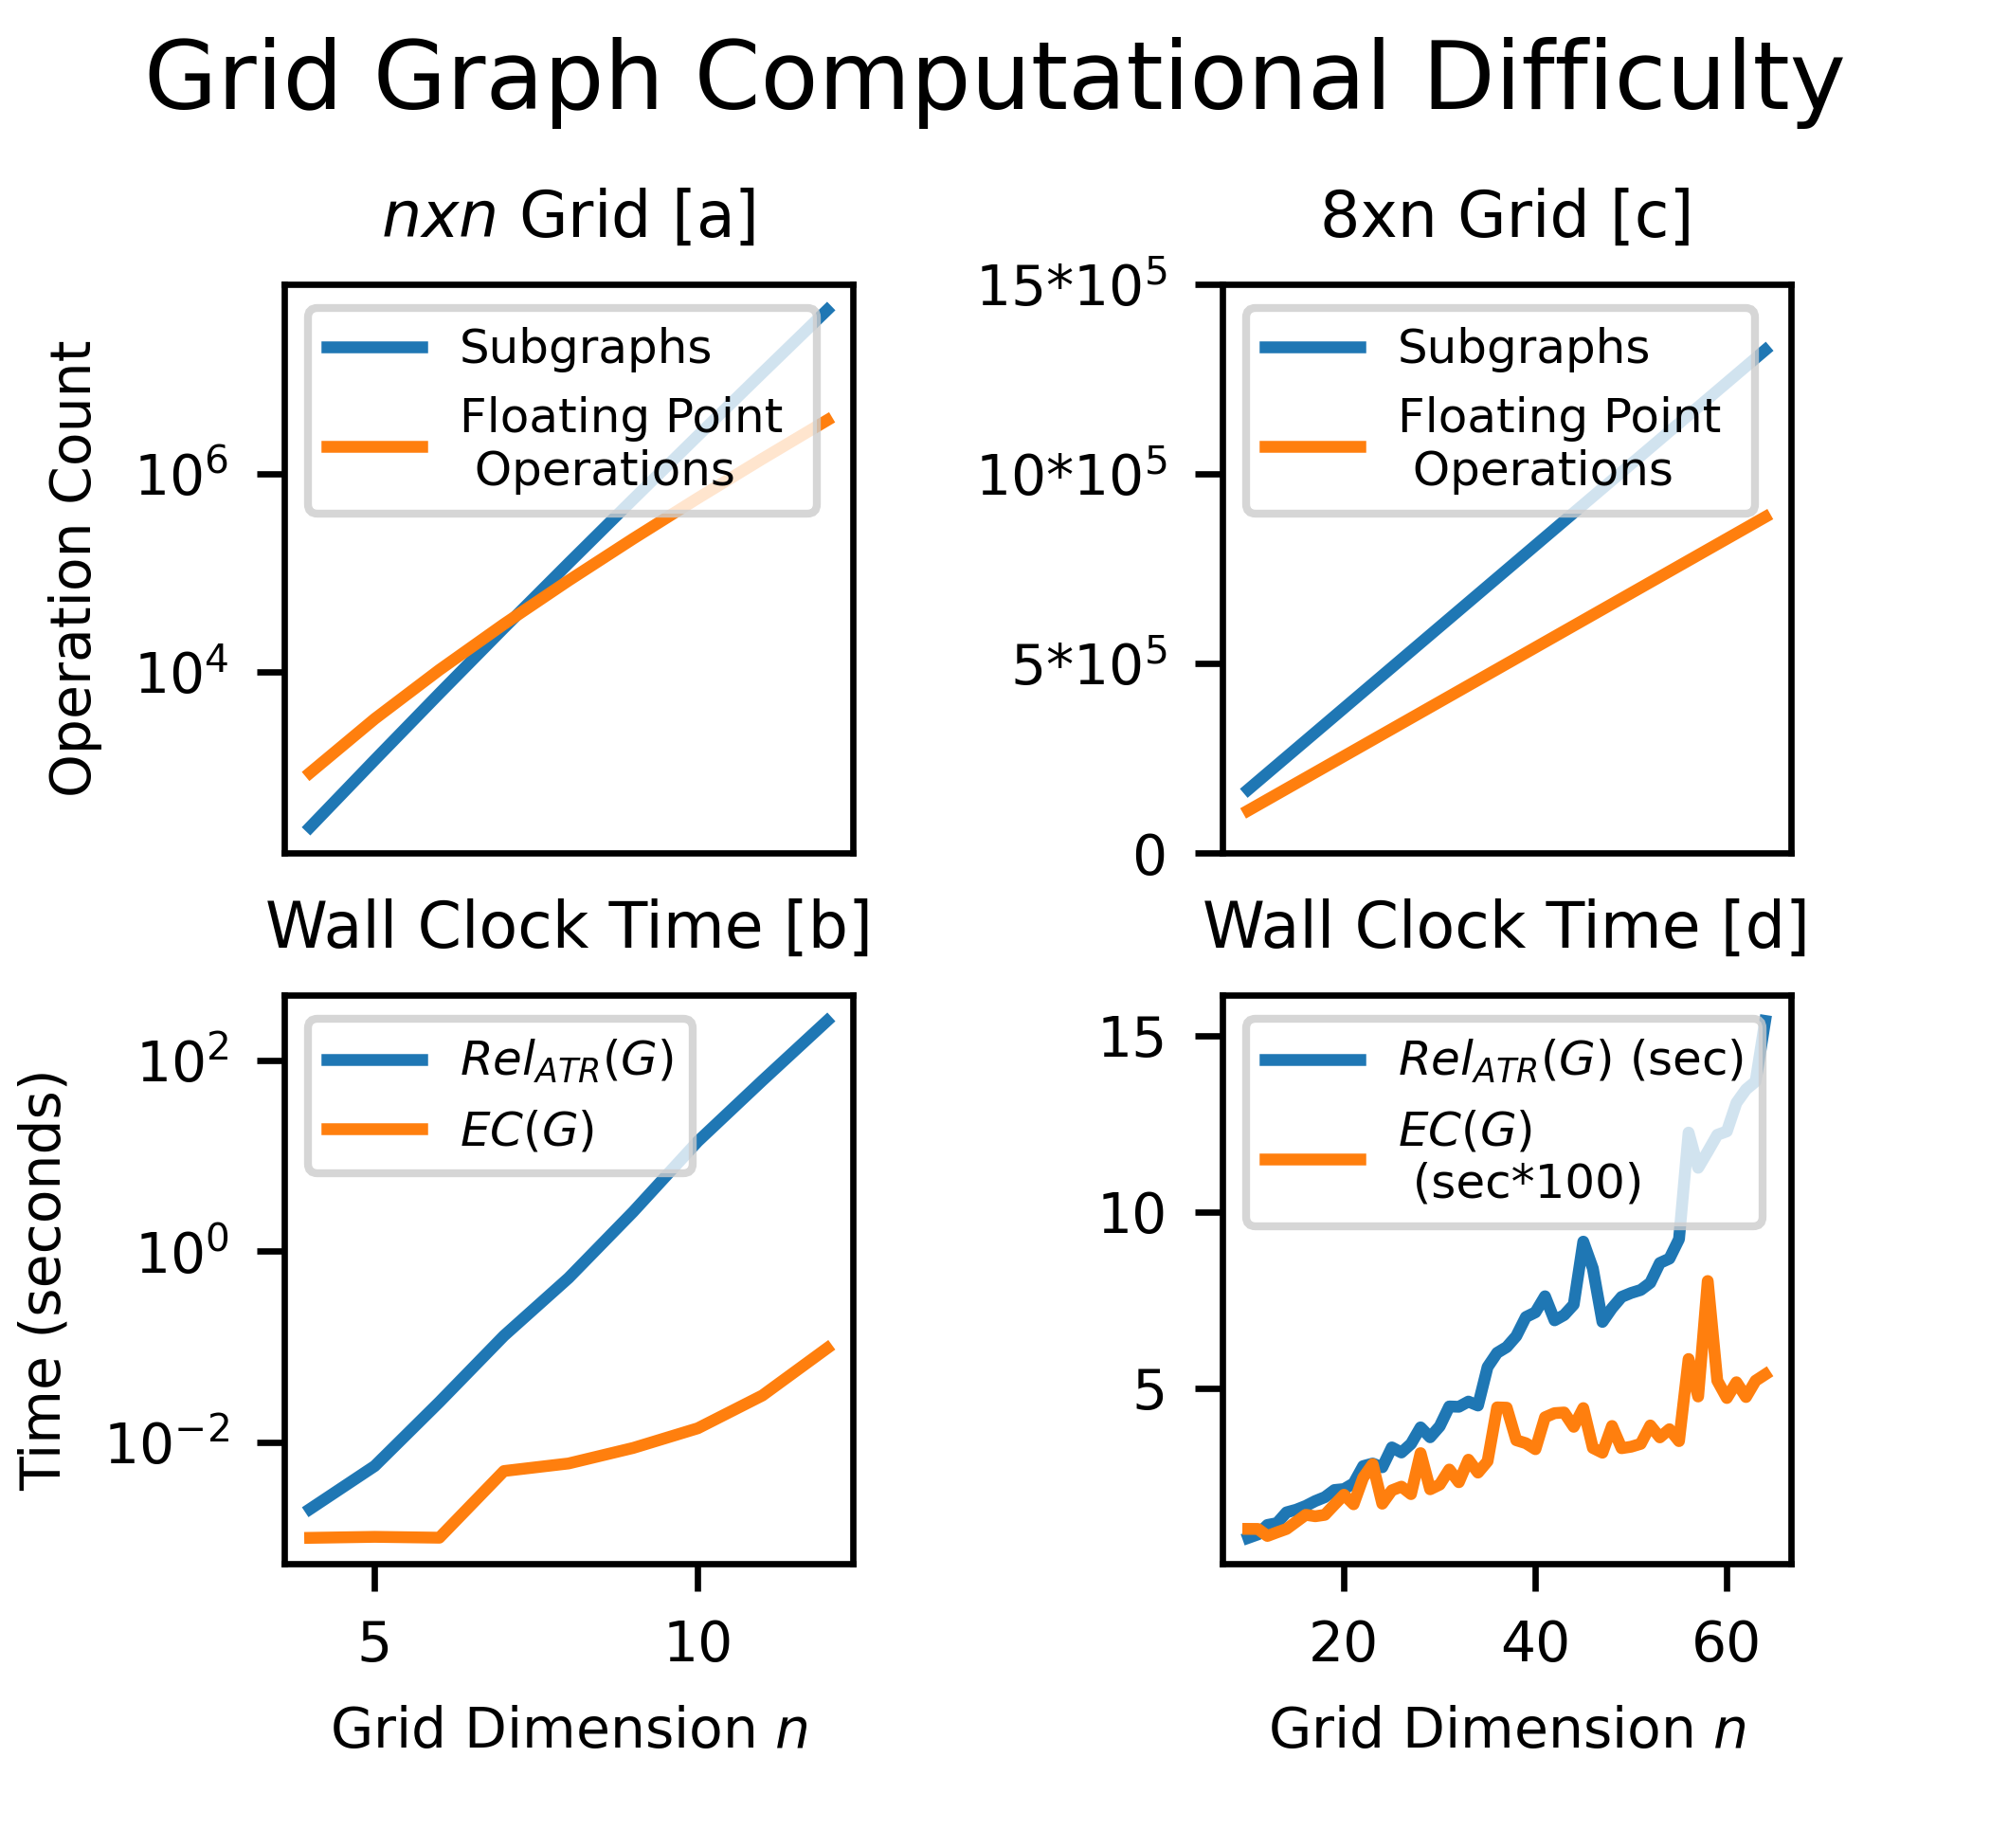
\includegraphics[width=0.5\textwidth]{../figures/GridGraphComputeTime8.png}
\end{figure}

\hypertarget{monte-carlo-mc-comparison}{%
\subsubsection{Monte Carlo (MC) Comparison}\label{monte-carlo-mc-comparison}}

As the TNC only bounds \(Rel_{ATR}(G)\) by calculating \(EC(G)\), we can evaluate the quality of this estimate by determining the number of MC trials needed to obtain bounds of \(Rel_{ATR}(G)\) better than \(EC(G)\). Using a 95\% confidence interval, we can calculate the number of MC trials needed to create a confidence interval that excludes \(EC(G)\).

For an edge failure rate of 0.01, both \(Rel_{ATR}(G)\) and \(EC(G)\) are approximately constant at 0.9996. Approximately 24 million MC trials are needed to rule out \(EC(G)\), and this count is insensitive to the size of the grid. Therefore, for reliable grid graphs, \(EC(G)\) is a good bound.

\hypertarget{random-connected-cubic-graphs}{%
\subsection{Random Connected Cubic Graphs}\label{random-connected-cubic-graphs}}

\hypertarget{computational-time-1}{%
\subsubsection{Computational Time}\label{computational-time-1}}

A random selection of 10,000 random connected cubic graphs \(G_{rc}\) from node count \(|N|=20\) to \(|N|=400\) were generated. The treewidth of \(G_{rc}\) and the treewidth of \(LG(G_{rc})\) were computed using an approximate treewidth solver \cite{dell2018pace} for 6 seconds. The pathwidth of \(G_{rc}\) was estimated from the tree decomposition of \(G_{rc}\). As seen in Figure \ref{fig:Random Cubic Treewidth}, there is a linear increase in approximated treewidth as graph size increases.

\begin{figure}[t]
\caption{Approximated treewidth, pathwidth, and treewidth of the line graph of $G_{rc}$ for 10,000 randomly generated connected cubic graphs $G_{rc}$, and the ratios between these widths.}
\label{fig:Random Cubic Treewidth}
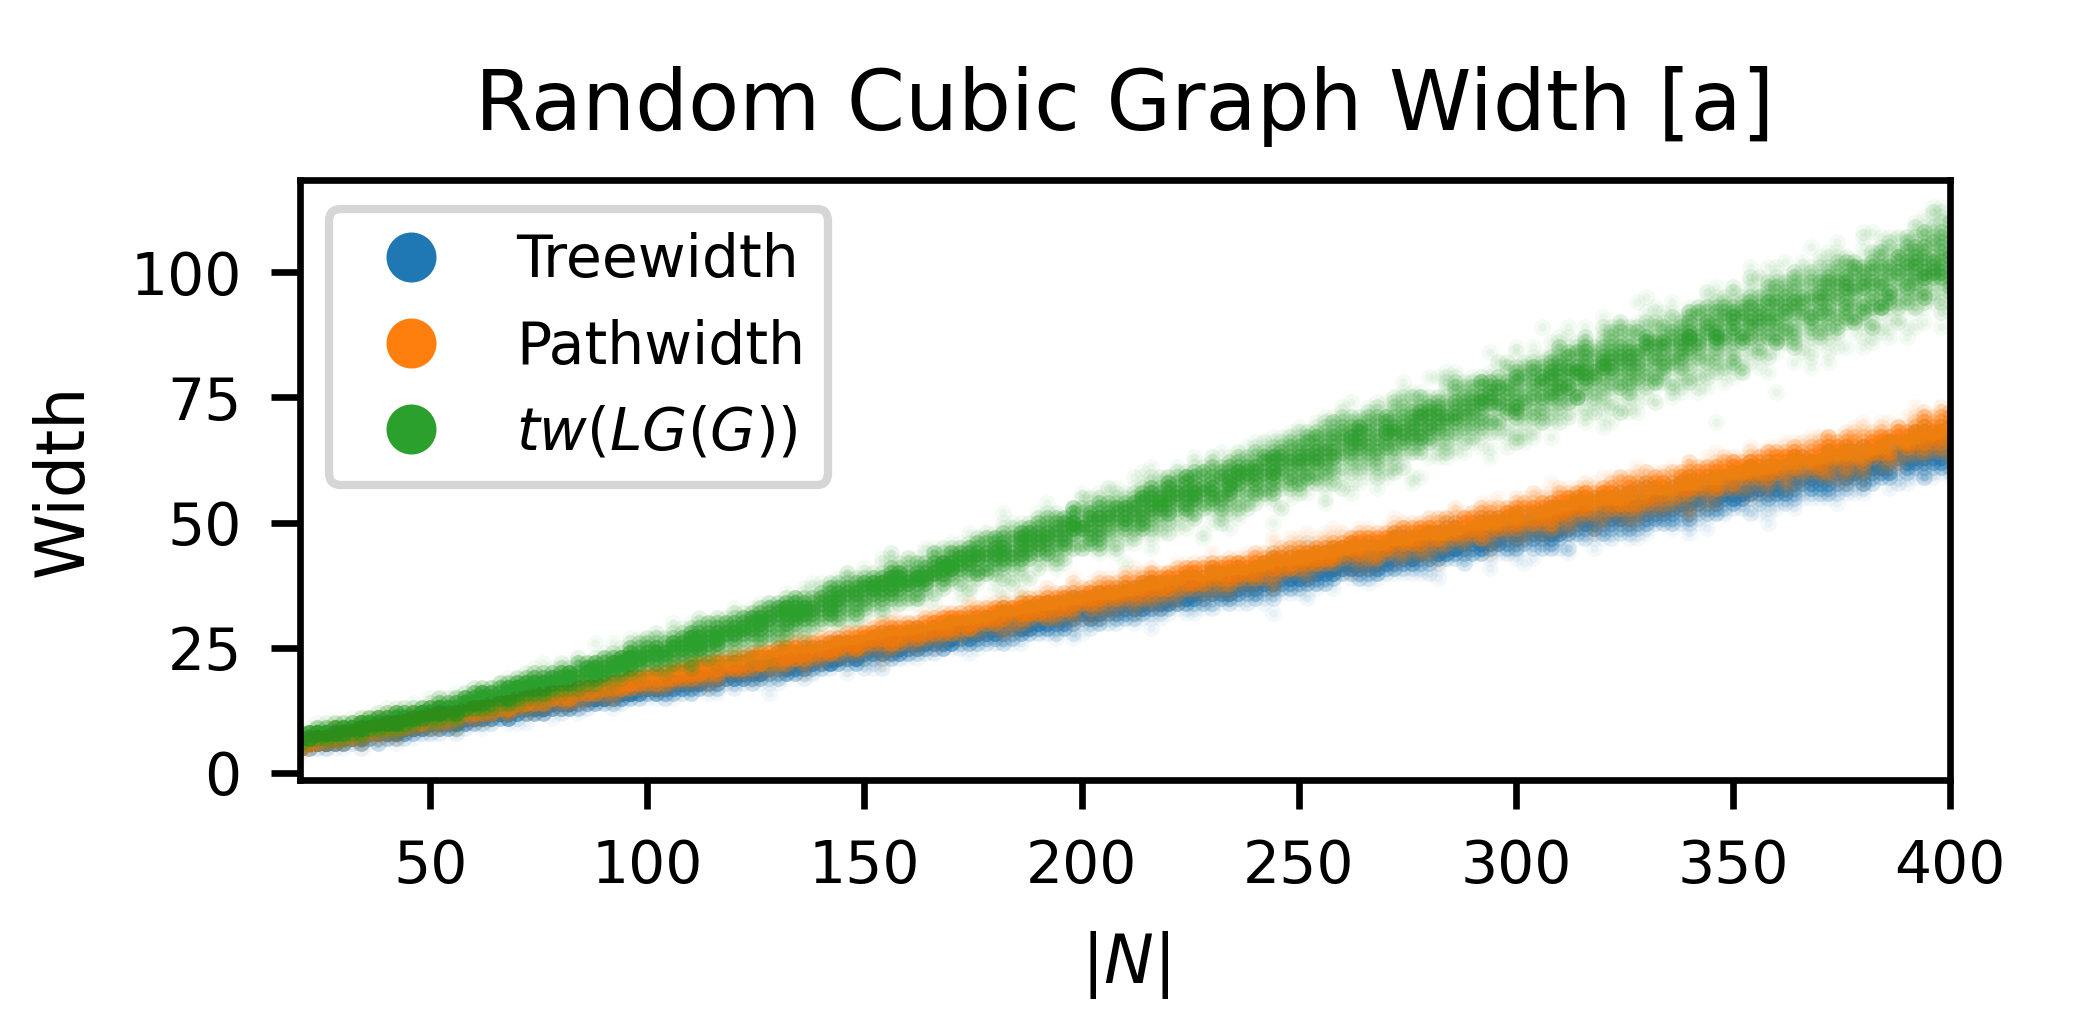
\includegraphics[width=0.5\textwidth]{../figures/RcubicWidth_short.png}
\end{figure}

\hypertarget{monte-carlo-mc-comparison-1}{%
\subsubsection{Monte Carlo (MC) Comparison}\label{monte-carlo-mc-comparison-1}}

A random selection of 10,000 random connected cubic graphs \(G_{rc}\) from node count \(|N|=20\) to \(|N|=50\) were generated and solved for \(EC(G)\) and \(Rel_{ATR}(G)\). Each edge had a failure rate of 0.01 to represent a network with high reliability. \(EC(G)\) is very tightly constrained, with a standard deviation of \(1.1*10^{-12}\) for all \textbar N\textbar, and can be estimated as \(EC(G) \approx (1-|N|*0.01^3)\). \(Rel_{ATR}(G)\) had greater variance, with a range of {[}0.92265,0.99998{]}.

For each graph, the number of MC trials needed to rule out the \(EC(G)\) bound at the 95\% confidence interval was calculated. Figure \ref{fig:Random Cubic MC} shows the proportion of cubic graphs that need less than \(X\) MC trials to rule out the \(EC(G)\) bound. The observed segmented stair-step pattern is unusual, and is likely caused by the graphs in each segment sharing some topological feature such as a bridge.

As graph size increases, the empirical cumulative distribution function pushes up and to the left, indicating more graphs need fewer MC trials to rule out the \(EC(G)\) bound. This means as highly reliable cubic graphs become larger, \(EC(G)\) becomes a worse bounding value of \(Rel_{ATR}(G)\).

\begin{figure}[t]
\caption{The empirical cumulative distribution function of randomly generated connected cubic graphs of size |N| that need less than $X$ MC trials of $Rel_{ATR}(G)$ to rule out the bound from $EC(G)$ at the 95\% confidence level.}
\label{fig:Random Cubic MC}
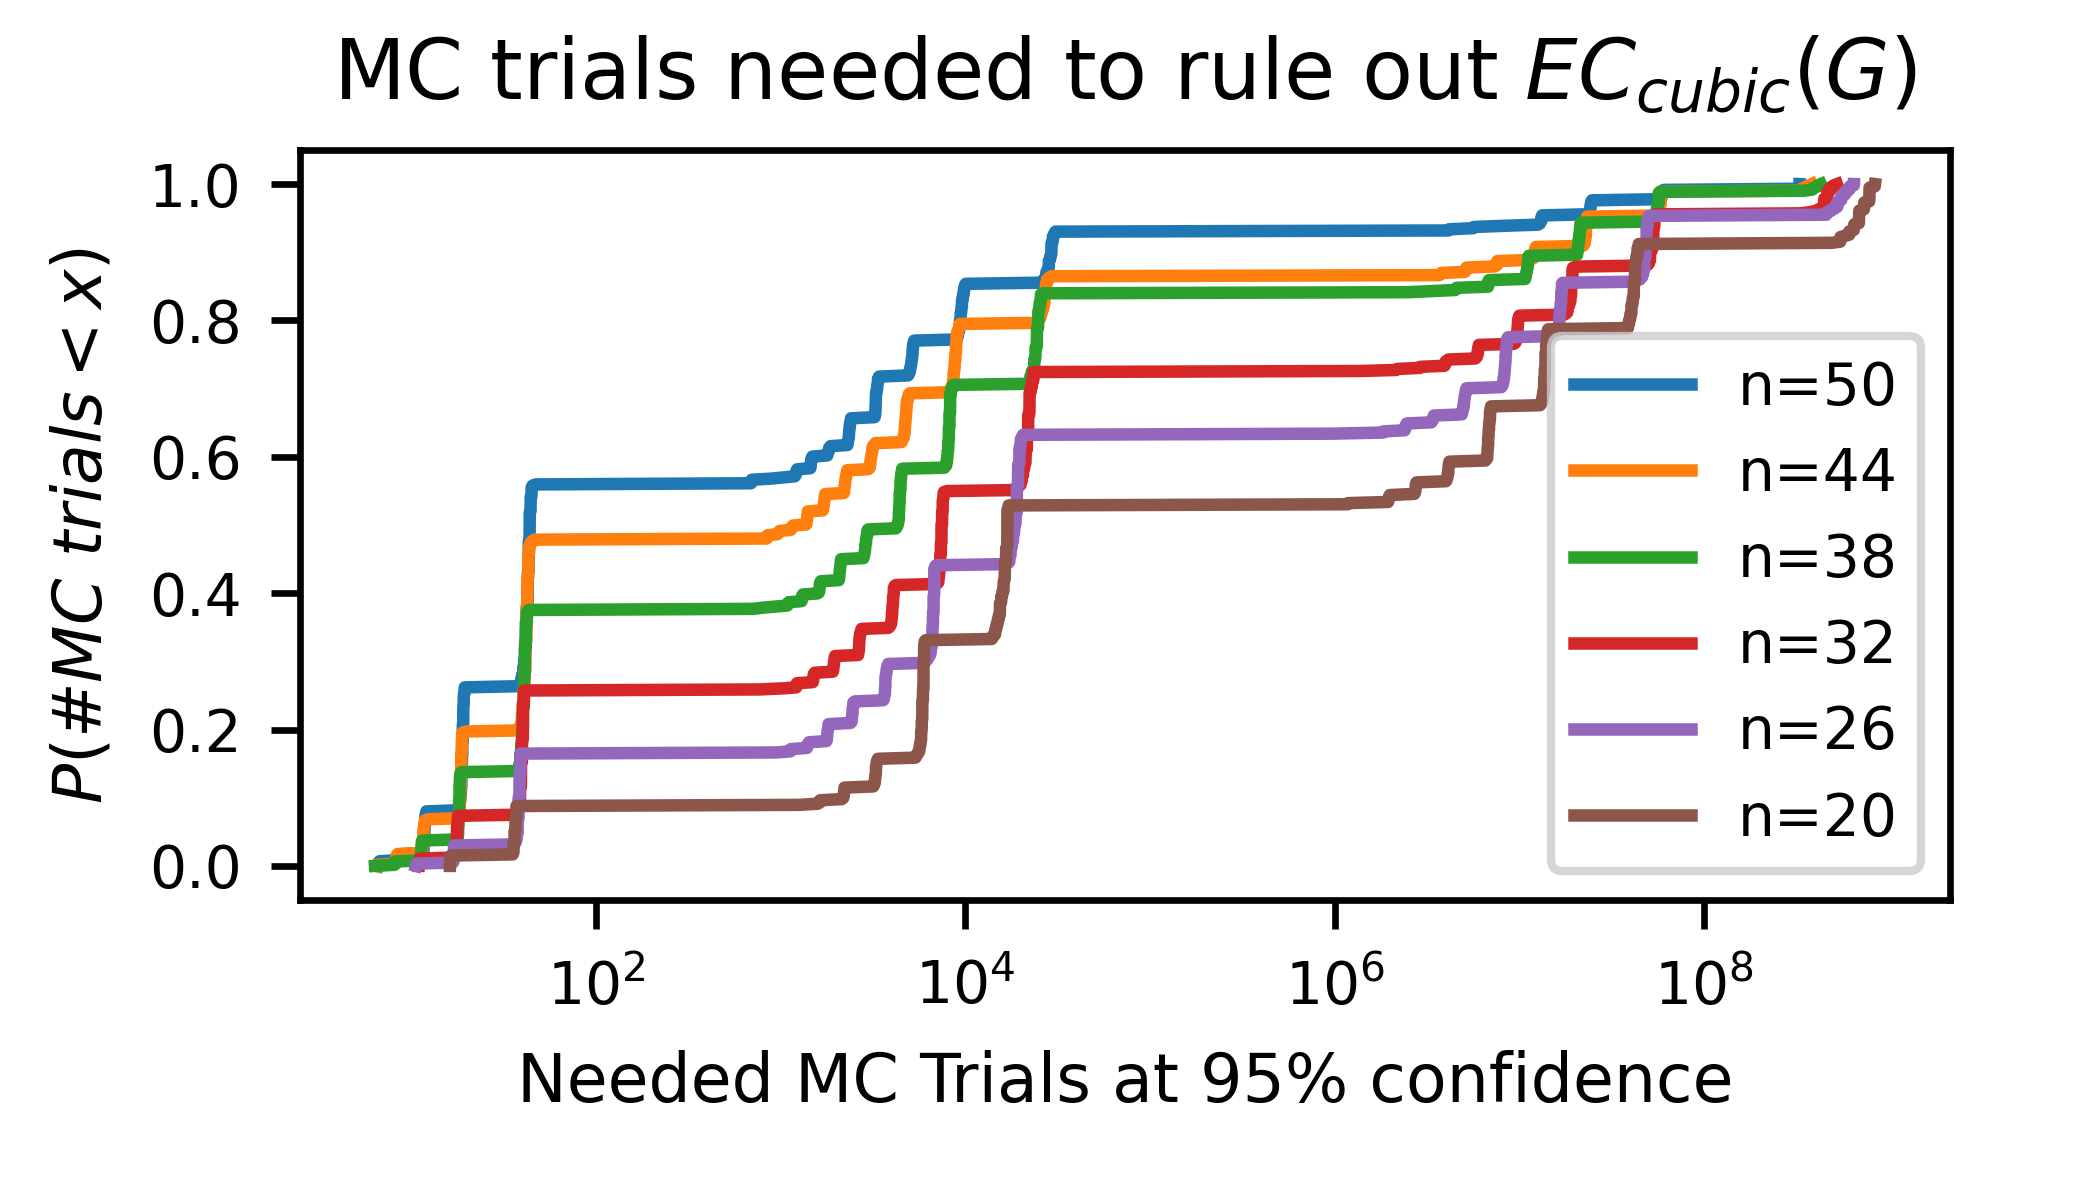
\includegraphics[width=0.5\textwidth]{../figures/RcubicTrials.png}
\end{figure}

Overall, despite the computational advantages of TNCs, the treewidth of these graphs scales linearly with size, resulting in computational complexity growing exponentially with the size of the graph. In addition, \(EC(G)\) as measured by TNCs is a poor bounding value for many cubic graphs, only a few MC trials are needed to achieve a better bounding value. This bounding value becomes worse as the graph size increases.

\hypertarget{power-transmission-grids}{%
\subsection{Power Transmission Grids}\label{power-transmission-grids}}

The \(Rel_{ATR}(G)\) and \(EC(G)\) of 58 transmission power grids \cite{li2016characterizing} were calculated. Table \ref{tab:Power Transmission Grid} shows the node and edge count of these graphs after reliability preserving reductions, and the result of the \(Rel_{ATR}(G)\) and \(EC(G)\) calculations at edge failure rate 0.5, 0.1 and 0.01. Some graphs were omitted due to trivial structure or inability to compute \(Rel_{ATR}(G)\).

Figure \ref{fig:Width Comparison} shows the treewidth and \(tw(LG(G))\) of the power grids in relation to the previously analyzed graphs. In general, the treewidth of the power grids is smaller than equal sized cubic graphs, making them very computationally efficient to solve. However, \(tw(LG(G))\) of the power grids are significantly greater than their treewidth, comparable to \(tw(LG(G_{rc}))\) of equal sized cubic graphs, due to the presence of high degree nodes in the power grids. The tensor factoring techniques in \cite{dudek2019efficient} may reduce these large values of \(tw(LG(G))\). Despite this, TNCs still quickly solve \(EC(G)\) and \(Rel_{S-T}(G)\) of these graphs in comparison to the binary decision diagram techniques.

\begin{figure}[t]
\caption{Treewidth and $tw(LG(G))$ comparison between grid graphs, random cubic graphs, and power transmission grids.}
\label{fig:Width Comparison}
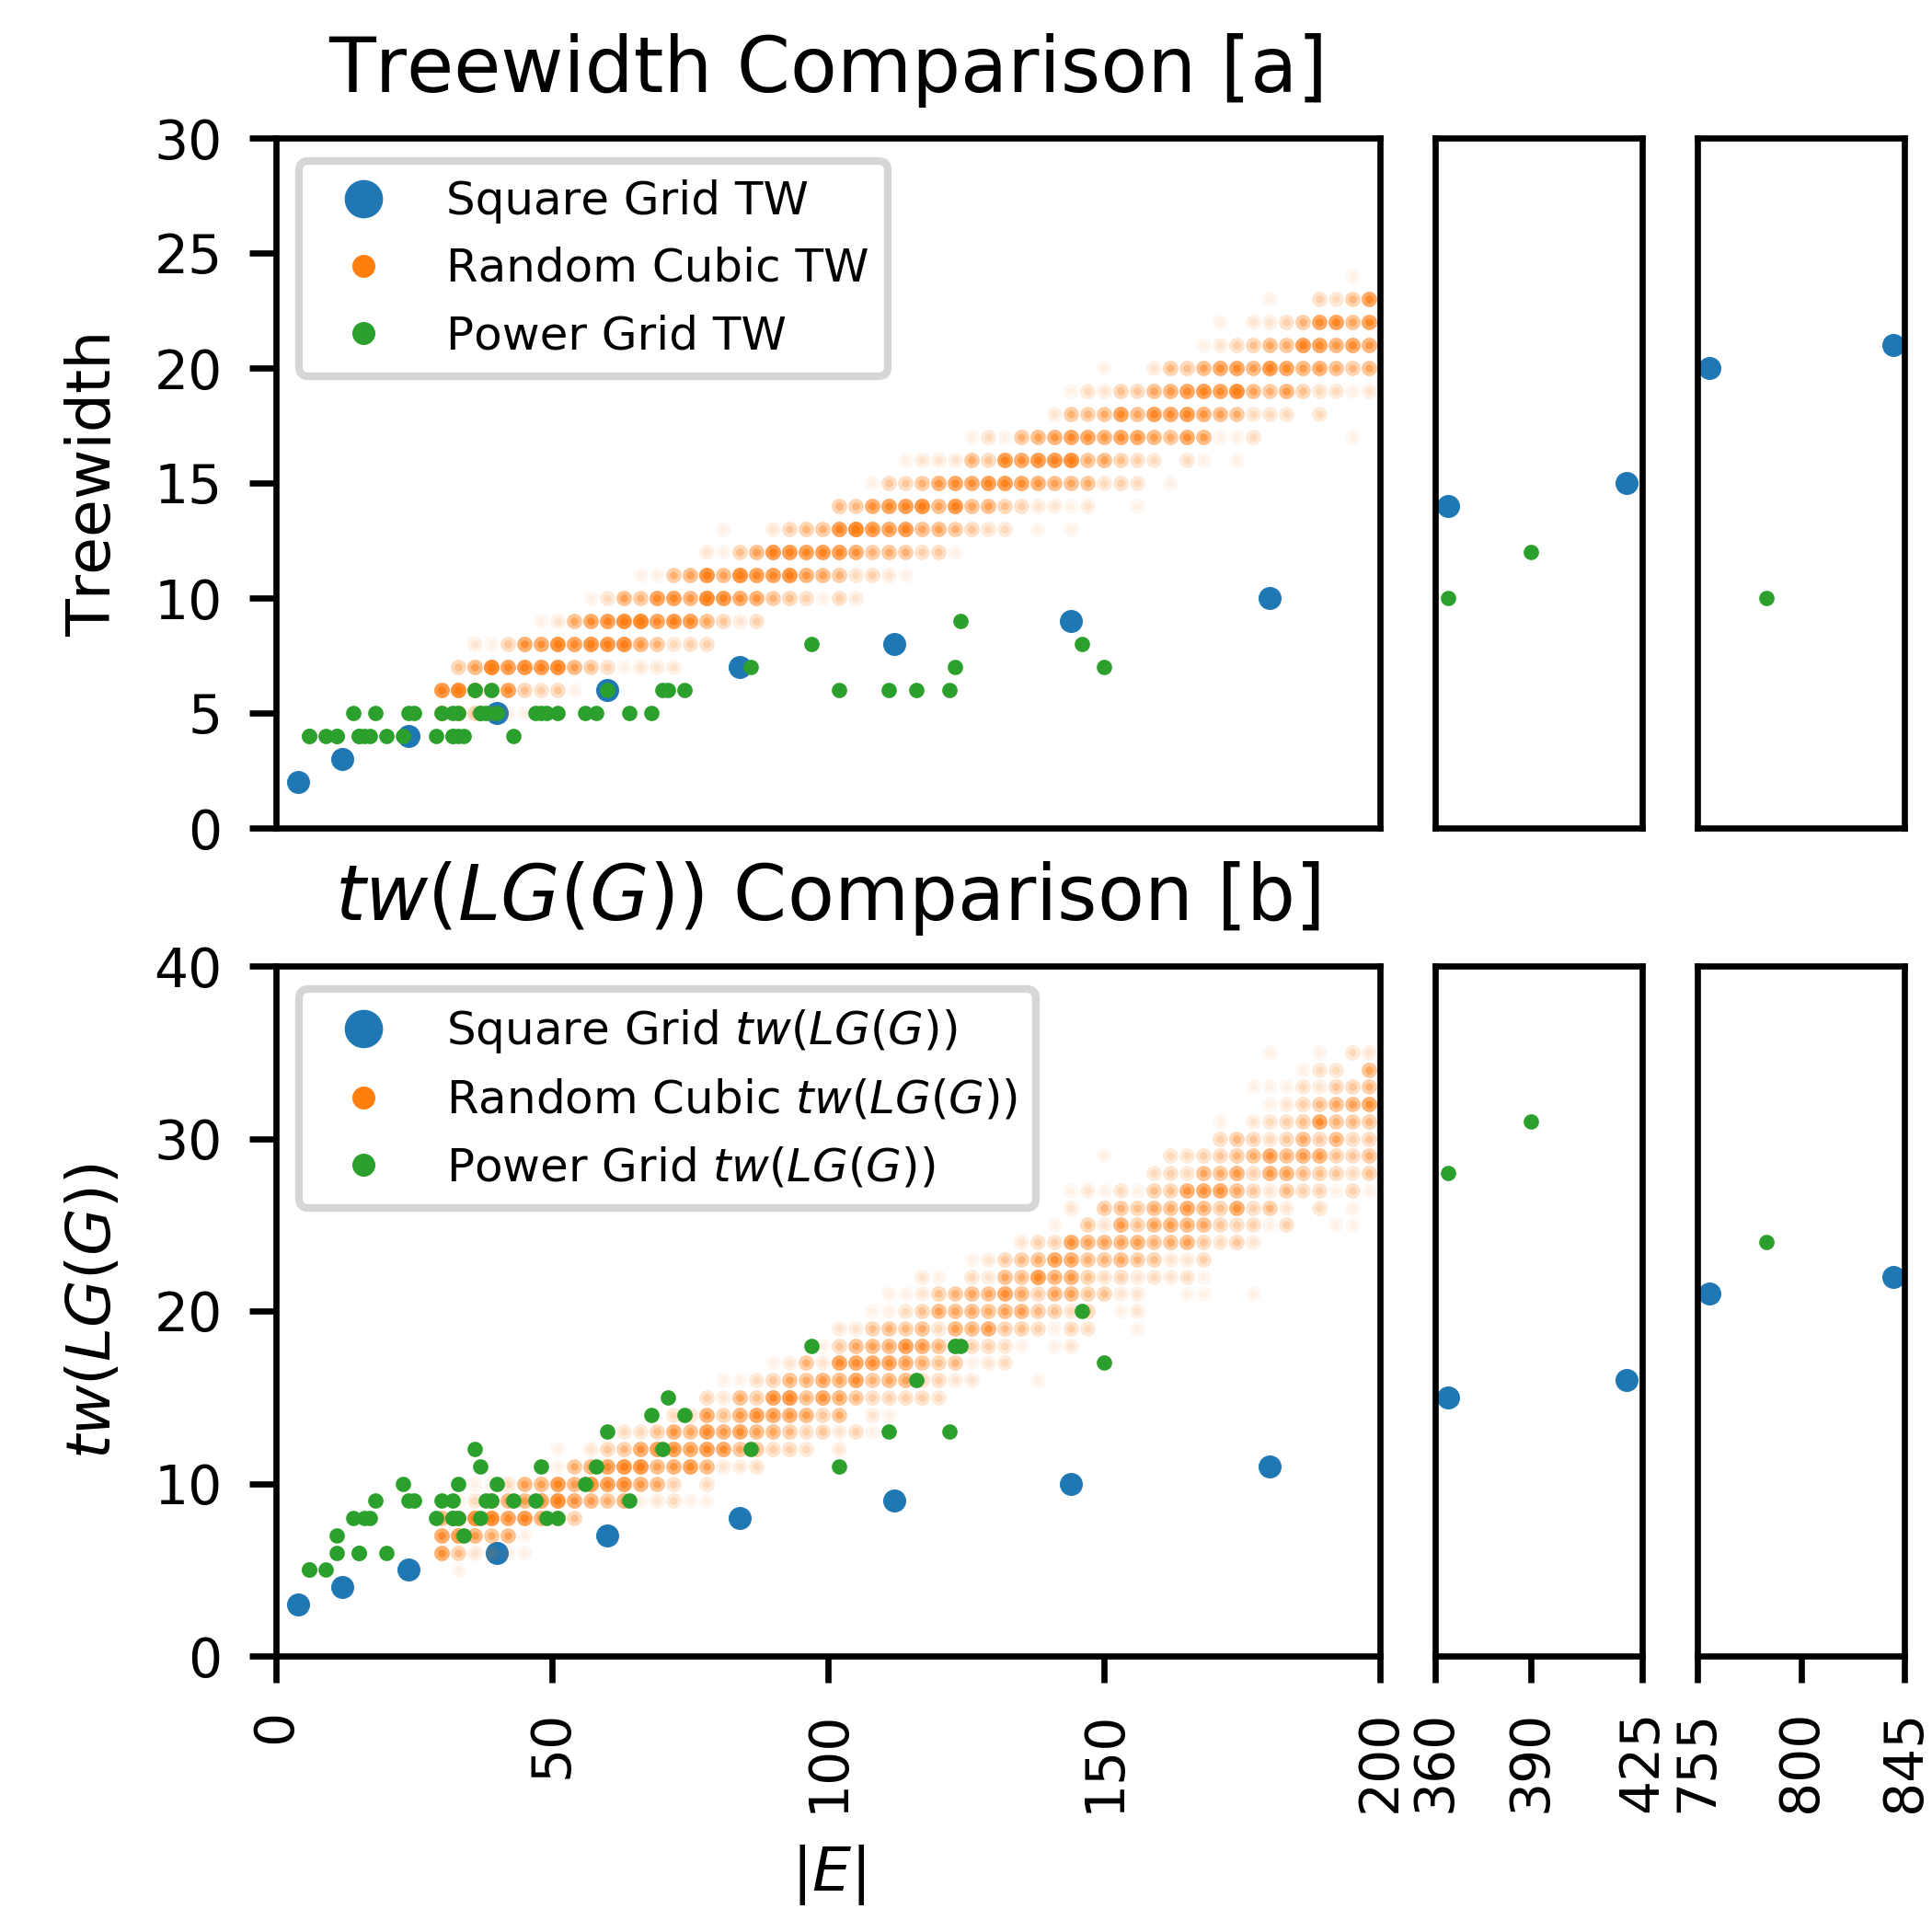
\includegraphics[width=0.5\textwidth]{../figures/WidthCompare.png}
\end{figure}

When each edge only has a 1\% chance of failure, \(EC(G)\) is a good approximation for 37 of the power grids as seen in the tall green bars in Figure \ref{fig:Power Grid MC}. It would take more than 1,000,000 MC trials to rule out the \(EC(G)\) approximation for these graphs. For the largest power grids, only 1,000 MC trials are needed to rule out \(EC(G)\).

\begin{figure}[t]
\caption{Number of MC Trials needed to rule out $EC(G)$ at the 95\% confidence level for each power grid at different edge failure rates $p$.}
\label{fig:Power Grid MC}
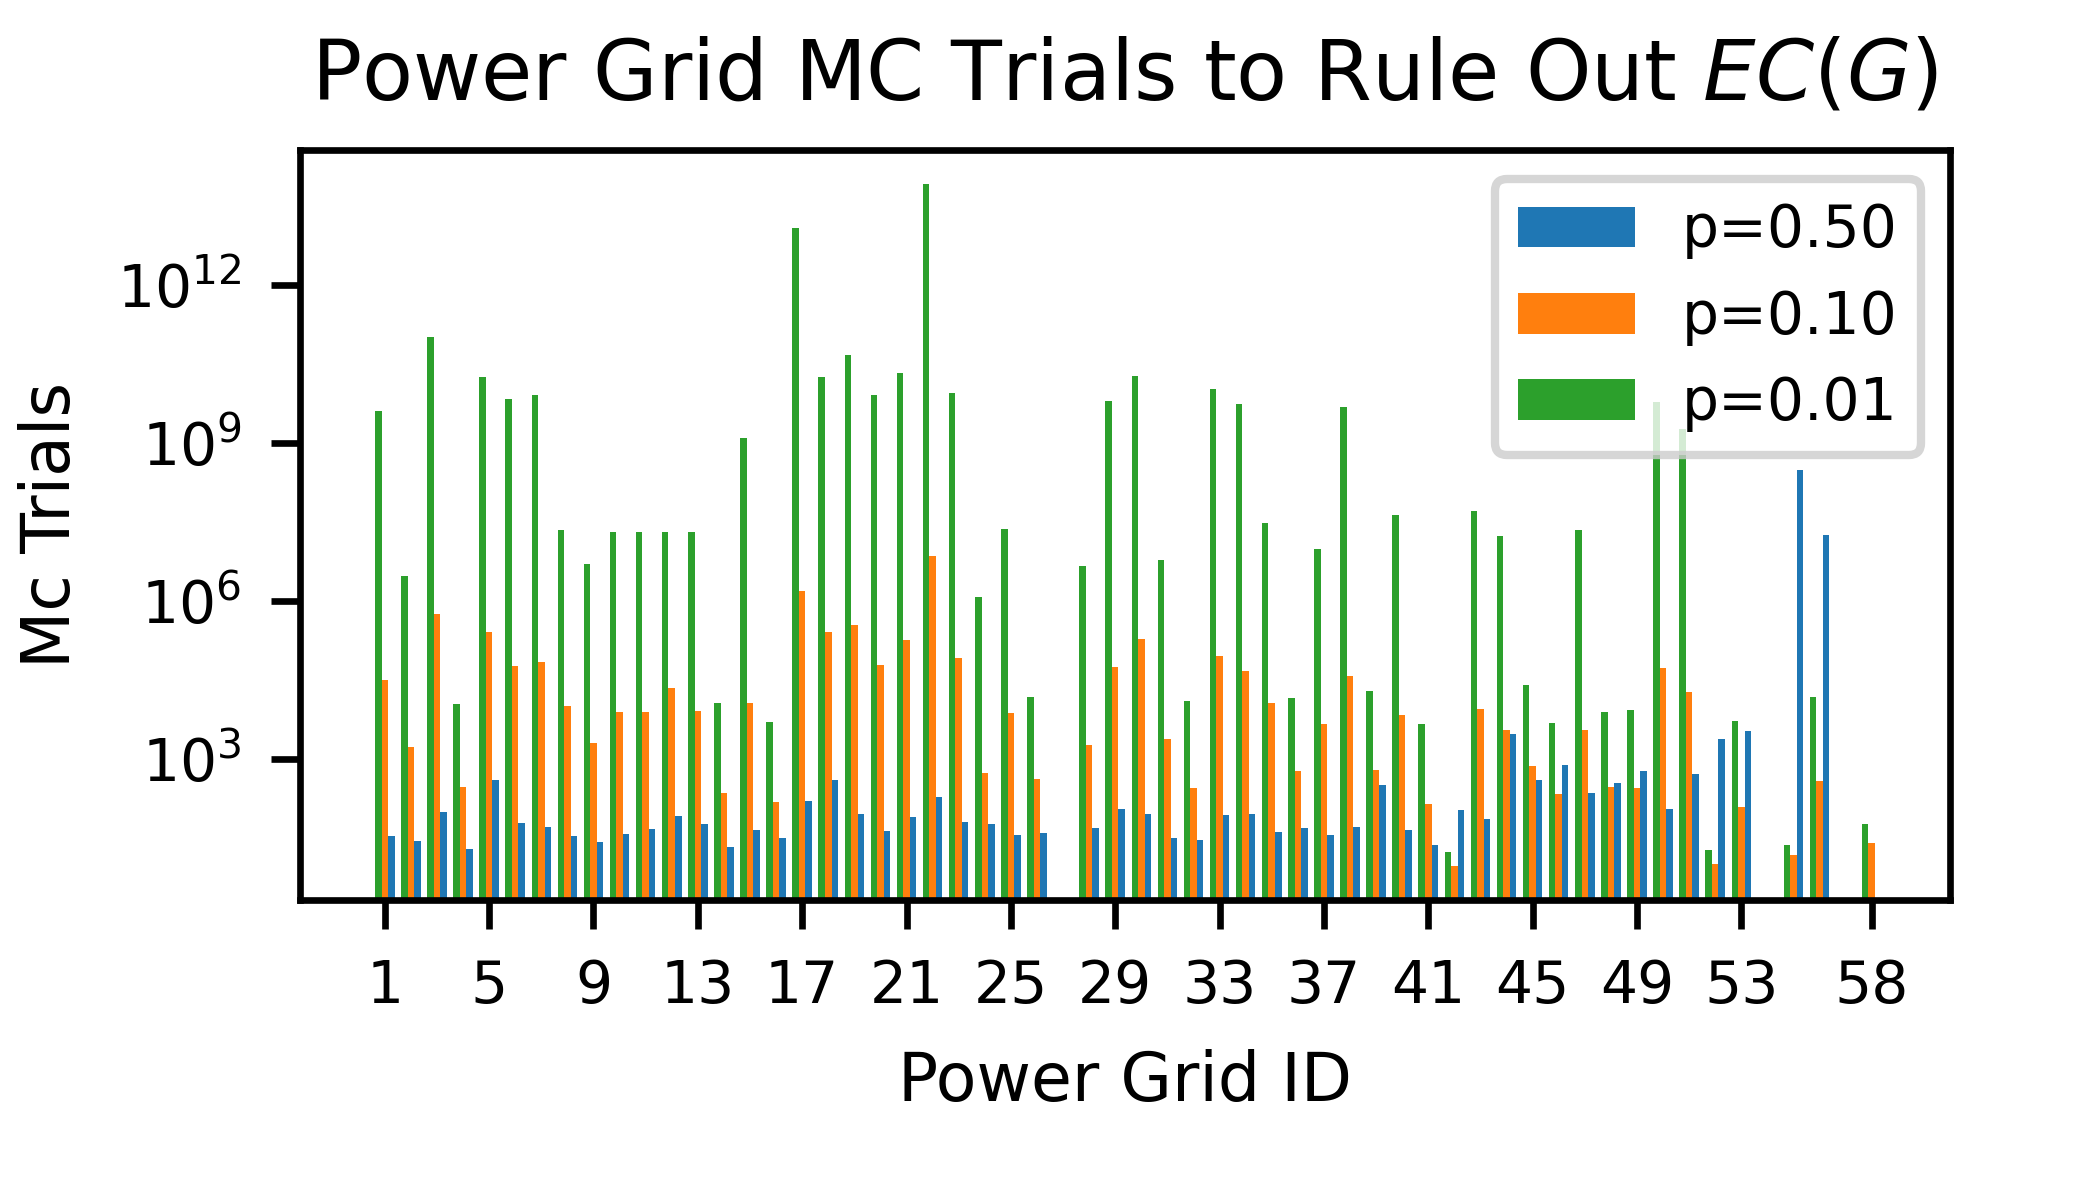
\includegraphics[width=0.5\textwidth]{../figures/PowerGridMC.png}
\end{figure}

\hypertarget{conclusion}{%
\section{Conclusion}\label{conclusion}}

\hypertarget{results-summary}{%
\subsection{Results Summary}\label{results-summary}}

Overall, TNCs for solving \(Rel_{S-T}(G)\) and estimating \(Rel_{ATR}(G)\) demonstrate many computational advantages on many practical networks. These methods are parameterized by the treewidth of the network, so graphs with low treewidth such as grids and the 58 power transmission networks can be quickly solved. In the general case as represented as random cubic graphs, TNCs are not as computationally efficient due to the linear relationship between treewidth and random cubic graph size. In addition, the presence of high degree nodes in the power transmission networks introduces a large constant factor between treewidth and the computationally relevant treewidth of the line graph. Despite these limitations, the tensor methods are still 10 to 100 times faster than the state-of-the-art binary decision diagram methods as measured by wall clock time.

When estimating \(Rel_{ATR}(G)\) by calculating \(EC(G)\), TNCs show excellent results on grid graphs. As edge failure rate decreases, as is the case for highly reliable networks, \(EC(G)\) becomes a better estimator. This increase in estimation accuracy is likely due to the fact that as edge failures become less likely, multiple edge failures needed to disconnect the graph become exponentially less likely, which heavily discounts occurrences of disconnected ``islands'' of nodes that satisfy \(EC(G)\) and do not satisfy \(Rel_{ATR}(G)\).

However, \(EC(G)\) is only a good estimate for \(Rel_{ATR}(G)\) for a small subset of cubic graphs and 37 out of 55 of the power grids. This work did not investigate why \(EC(G)\) was a good estimate for these graphs, although it is likely due to topological bottlenecking effects.

\hypertarget{future-work}{%
\subsection{Future Work}\label{future-work}}

In relation to algorithm design, the primary bottleneck to TNCs is the memory requirement. Techniques such as sparse arrays, online matrix compression, or tensor factoring can be used to reduce the memory footprint of large tensors. Additionally, many quantum computer algorithms can be described as tensor contractions \cite{biamonte2017tensor} \cite{duenas2018quantum}, so these TNCs may be able to exploit quantum computers to achieve a quantum speedup over traditional algorithms.

As \(EC(G)\) is not always a good approximation for \(Rel_{ATR}(G)\), it would be beneficial to classify the graphs where \(EC(G)\) is a good approximation of \(Rel_{ATR}(G)\). If an algorithm can quickly identify these classes of graphs, then tensor methods can quickly and confidently estimate \(Rel_{ATR}(G)\) using \(EC(G)\). In addition, determining how to incorporate TNCs with other \#SAT solvers into a virtual best solver will greatly expand the classes of graphs where \(EC(G)\) can be quickly solved.

While \(Rel_{S-T}(G)\) can be exactly solved by tensor methods for directed acyclic graphs, the introduction of cycles causes drastic multiplicative overcounting of solutions if the given \(Rel_{S-T}(G)\) formulation is used. Determining a better tensor graph for solving \(Rel_{S-T}(G)\) or determining how to compensate for the multiplicative overcounting can expand the number of graphs that can be exactly solved by TNCs.

\begin{table*}[ht]
\centering
\caption{Power Transmission Network Attributes}
\label{tab:Power Transmission Grid}
\newcolumntype{a}{X}
\newcolumntype{b}{>{\hsize=.33\hsize}X}
\renewcommand{\arraystretch}{.75}
\begin{tabularx}{\textwidth}{bbbbbbaaaaaaaa}
\toprule
ID & |V| & |E| & TW & PW & LGW & $Rel_{time}$ & $Rel_{0.5}$ & $Rel_{0.1}$ & $Rel_{0.01}$ & $EC_{time}$ & $EC_{0.5}$ & $EC_{0.1}$ & $EC_{0.01}$ \tabularnewline
\midrule
% flatex input: [../tables/PowerGridsRELTable.tex]
1 & 16 & 29 & 4 & 5 & 8 & 0.017332 & 0.12167154 & 0.98957460 & 0.99999087 & 0.174876 & 0.25502051 & 0.99065582 & 0.99999096 \tabularnewline
2 & 19 & 33 & 4 & 4 & 8 & 0.000186 & 0.05365770 & 0.98211723 & 0.99998379 & 0.000333 & 0.17822816 & 0.98764111 & 0.99998795 \tabularnewline
3 & 9 & 18 & 5 & 5 & 9 & 0.000597 & 0.42333221 & 0.99636464 & 0.99999694 & 0.000723 & 0.52156830 & 0.99651838 & 0.99999695 \tabularnewline
4 & 12 & 20 & 4 & 4 & 6 & 0.000000 & 0.12807083 & 0.97834075 & 0.99988980 & 0.000172 & 0.31490231 & 0.99091973 & 0.99999098 \tabularnewline
5 & 4 & 6 & 4 & 3 & 5 & 0.000000 & 0.59375000 & 0.99581400 & 0.99999597 & 0.000000 & 0.64062500 & 0.99605700 & 0.99999600 \tabularnewline
6 & 24 & 48 & 5 & 6 & 11 & 0.004095 & 0.06873492 & 0.98659392 & 0.99998786 & 0.000753 & 0.15051040 & 0.98749687 & 0.99998794 \tabularnewline
7 & 13 & 24 & 5 & 5 & 9 & 0.004037 & 0.19829893 & 0.99110197 & 0.99999191 & 0.000333 & 0.31878930 & 0.99177120 & 0.99999197 \tabularnewline
8 & 16 & 32 & 5 & 5 & 9 & 0.004749 & 0.16953775 & 0.99180050 & 0.99999289 & 0.000913 & 0.31583457 & 0.99342016 & 0.99999394 \tabularnewline
9 & 19 & 34 & 4 & 4 & 7 & 0.000333 & 0.05261123 & 0.98166897 & 0.99998374 & 0.001684 & 0.17841807 & 0.98687403 & 0.99998697 \tabularnewline
10 & 9 & 15 & 4 & 4 & 6 & 0.000000 & 0.27203369 & 0.99197148 & 0.99999289 & 0.000256 & 0.42657471 & 0.99376760 & 0.99999397 \tabularnewline
11 & 7 & 11 & 4 & 3 & 6 & 0.000000 & 0.34082031 & 0.99218972 & 0.99999290 & 0.000513 & 0.48193359 & 0.99398015 & 0.99999399 \tabularnewline
12 & 17 & 36 & 6 & 6 & 12 & 0.023612 & 0.22980855 & 0.99329227 & 0.99999393 & 0.002440 & 0.32829193 & 0.99430582 & 0.99999493 \tabularnewline
13 & 6 & 9 & 4 & 3 & 5 & 0.000333 & 0.38671875 & 0.99237749 & 0.99999291 & 0.000334 & 0.51367188 & 0.99409283 & 0.99999400 \tabularnewline
14 & 18 & 32 & 4 & 3 & 8 & 0.000342 & 0.05216674 & 0.97114616 & 0.99988185 & 0.000333 & 0.19721385 & 0.98784985 & 0.99998797 \tabularnewline
15 & 23 & 39 & 6 & 6 & 9 & 0.005238 & 0.02955951 & 0.97957456 & 0.99998174 & 0.000927 & 0.10569971 & 0.98202115 & 0.99998197 \tabularnewline
16 & 23 & 40 & 5 & 6 & 10 & 0.003775 & 0.02555826 & 0.96167545 & 0.99978280 & 0.000506 & 0.12043086 & 0.98454274 & 0.99998493 \tabularnewline
17 & 6 & 11 & 4 & 3 & 7 & 0.000000 & 0.55371094 & 0.99753011 & 0.99999796 & 0.000336 & 0.62939453 & 0.99760764 & 0.99999796 \tabularnewline
18 & 4 & 6 & 4 & 3 & 5 & 0.000000 & 0.59375000 & 0.99581400 & 0.99999597 & 0.000000 & 0.64062500 & 0.99605700 & 0.99999600 \tabularnewline
19 & 9 & 17 & 4 & 4 & 8 & 0.000269 & 0.36923218 & 0.99458268 & 0.99999496 & 0.000000 & 0.47051239 & 0.99482186 & 0.99999498 \tabularnewline
20 & 16 & 30 & 5 & 5 & 9 & 0.002691 & 0.14746502 & 0.99081730 & 0.99999189 & 0.001519 & 0.27150461 & 0.99154743 & 0.99999195 \tabularnewline
21 & 18 & 37 & 5 & 5 & 11 & 0.002053 & 0.16092585 & 0.99022499 & 0.99999092 & 0.000337 & 0.25048232 & 0.99066939 & 0.99999096 \tabularnewline
22 & 7 & 14 & 5 & 4 & 8 & 0.001577 & 0.55395508 & 0.99764972 & 0.99999797 & 0.000501 & 0.62353516 & 0.99768485 & 0.99999797 \tabularnewline
23 & 9 & 16 & 4 & 3 & 8 & 0.000250 & 0.31793213 & 0.99331619 & 0.99999393 & 0.003037 & 0.43721008 & 0.99385534 & 0.99999398 \tabularnewline
24 & 31 & 51 & 5 & 5 & 8 & 0.004045 & 0.00333280 & 0.96024725 & 0.99996437 & 0.003970 & 0.04349889 & 0.97436290 & 0.99997398 \tabularnewline
25 & 9 & 15 & 4 & 3 & 6 & 0.000757 & 0.25952148 & 0.99102678 & 0.99999189 & 0.000000 & 0.41384888 & 0.99297602 & 0.99999299 \tabularnewline
26 & 27 & 49 & 5 & 5 & 8 & 0.001722 & 0.01736987 & 0.96797843 & 0.99987974 & 0.000333 & 0.09222602 & 0.98204488 & 0.99998198 \tabularnewline
28 & 27 & 47 & 5 & 6 & 9 & 0.006189 & 0.01239560 & 0.97220986 & 0.99997466 & 0.000000 & 0.07123664 & 0.97908383 & 0.99997897 \tabularnewline
29 & 34 & 71 & 6 & 7 & 15 & 0.046117 & 0.02852902 & 0.98122226 & 0.99998281 & 0.019774 & 0.07020389 & 0.98231394 & 0.99998291 \tabularnewline
30 & 12 & 23 & 4 & 5 & 10 & 0.002861 & 0.24995208 & 0.99155426 & 0.99999195 & 0.000594 & 0.34471893 & 0.99195646 & 0.99999199 \tabularnewline
31 & 21 & 37 & 5 & 5 & 8 & 0.000335 & 0.03919450 & 0.97994898 & 0.99998177 & 0.000334 & 0.14345905 & 0.98499664 & 0.99998498 \tabularnewline
32 & 19 & 33 & 5 & 5 & 10 & 0.003519 & 0.04548891 & 0.96999886 & 0.99988083 & 0.000334 & 0.15963011 & 0.98581925 & 0.99998596 \tabularnewline
33 & 29 & 60 & 6 & 8 & 13 & 0.044070 & 0.04883569 & 0.98456505 & 0.99998585 & 0.005141 & 0.10738096 & 0.98535319 & 0.99998592 \tabularnewline
34 & 36 & 70 & 6 & 7 & 12 & 0.049390 & 0.01668428 & 0.97998377 & 0.99998179 & 0.002529 & 0.05712185 & 0.98122264 & 0.99998190 \tabularnewline
35 & 14 & 25 & 5 & 5 & 9 & 0.002144 & 0.15695018 & 0.98911478 & 0.99998990 & 0.000334 & 0.28797701 & 0.99087288 & 0.99999098 \tabularnewline
36 & 29 & 56 & 5 & 6 & 10 & 0.007635 & 0.02254811 & 0.97219655 & 0.99988380 & 0.001594 & 0.08928589 & 0.98340645 & 0.99998392 \tabularnewline
37 & 20 & 38 & 5 & 5 & 9 & 0.004598 & 0.07215021 & 0.98532712 & 0.99998682 & 0.003260 & 0.18448659 & 0.98851388 & 0.99998894 \tabularnewline
38 & 31 & 64 & 5 & 6 & 9 & 0.002900 & 0.03717040 & 0.98529150 & 0.99998684 & 0.001087 & 0.11263403 & 0.98646343 & 0.99998694 \tabularnewline
39 & 61 & 124 & 9 & 10 & 18 & 1.551559 & 0.00116882 & 0.95569496 & 0.99986768 & 0.047763 & 0.00951425 & 0.96999788 & 0.99997085 \tabularnewline
40 & 23 & 43 & 4 & 4 & 9 & 0.003473 & 0.03814892 & 0.98081026 & 0.99998276 & 0.000774 & 0.12076441 & 0.98385333 & 0.99998396 \tabularnewline
41 & 18 & 32 & 4 & 4 & 8 & 0.003706 & 0.05750333 & 0.96609719 & 0.99978686 & 0.000333 & 0.19745638 & 0.98784986 & 0.99998797 \tabularnewline
42 & 36 & 68 & 5 & 5 & 14 & 0.006670 & 0.00381684 & 0.81463673 & 0.98037497 & 0.007386 & 0.02868238 & 0.97142746 & 0.99997098 \tabularnewline
43 & 31 & 58 & 5 & 7 & 11 & 0.027855 & 0.01692225 & 0.97759178 & 0.99997973 & 0.003529 & 0.06477194 & 0.98050149 & 0.99998092 \tabularnewline
44 & 78 & 150 & 7 & 10 & 17 & 0.459141 & 0.00003289 & 0.93844113 & 0.99994142 & 0.076132 & 0.00077407 & 0.94594519 & 0.99994492 \tabularnewline
45 & 55 & 102 & 6 & 9 & 11 & 0.101259 & 0.00035646 & 0.94503474 & 0.99985754 & 0.002354 & 0.00611823 & 0.95975279 & 0.99995896 \tabularnewline
46 & 60 & 116 & 6 & 7 & 16 & 0.081021 & 0.00023098 & 0.92515124 & 0.99965566 & 0.026080 & 0.00335799 & 0.95504980 & 0.99995397 \tabularnewline
47 & 48 & 86 & 7 & 8 & 12 & 0.075847 & 0.00080723 & 0.95996061 & 0.99996351 & 0.001003 & 0.01131853 & 0.96602777 & 0.99996592 \tabularnewline
48 & 52 & 97 & 8 & 10 & 18 & 0.528176 & 0.00066992 & 0.93887114 & 0.99975969 & 0.100093 & 0.00760182 & 0.96237592 & 0.99996194 \tabularnewline
49 & 60 & 111 & 6 & 8 & 13 & 0.130469 & 0.00014183 & 0.93194376 & 0.99975358 & 0.008036 & 0.00387670 & 0.95751108 & 0.99995693 \tabularnewline
50 & 36 & 74 & 6 & 7 & 14 & 0.072151 & 0.02141654 & 0.97943954 & 0.99998083 & 0.006922 & 0.05905184 & 0.98061142 & 0.99998094 \tabularnewline
51 & 58 & 123 & 7 & 8 & 18 & 0.167014 & 0.00129092 & 0.96131942 & 0.99996365 & 0.095085 & 0.00715189 & 0.96402050 & 0.99996392 \tabularnewline
52 & 77 & 146 & 8 & 10 & 20 & 2.546974 & 0.00002134 & 0.76559700 & 0.97996221 & 0.214653 & 0.00090534 & 0.94845804 & 0.99994788 \tabularnewline
53 & 73 & 122 & 6 & 7 & 13 & 0.121916 & 0.00000214 & 0.89256304 & 0.99962324 & 0.009748 & 0.00057446 & 0.93907596 & 0.99993696 \tabularnewline
55 & 208 & 390 & 12 & 14 & 31 & 649.388035 & 0.00000000 & 0.66512161 & 0.97965552 & 313.083091 & 0.00000001 & 0.86434283 & 0.99985575 \tabularnewline
56 & 184 & 364 & 10 & 14 & 28 & 93.468759 & 0.00000000 & 0.85395647 & 0.99967281 & 97.081757 & 0.00000011 & 0.88667166 & 0.99988172 \tabularnewline
58 & 406 & 785 & 10 & 15 & 24 & 293.777338 & 0.00000000 & 0.56241914 & 0.98813658 & 12.744727 & 0.00000000 & 0.74302255 & 0.99970647 \tabularnewline

% flatex input end: [../tables/PowerGridsRELTable.tex]

%
\bottomrule
\end{tabularx}
\end{table*}

% flatex input end: [manuscript.tex]

% Here start your contexts...
% Here start your contexts...

\newpage
\clearpage
\section{REFERENCES}
{\small
%*flatex input: [ICOSSAR_2021_template.bbl]
\begin{thebibliography}{10}

\bibitem{valiant1979complexity}
Leslie~G Valiant.
\newblock The complexity of enumeration and reliability problems.
\newblock {\em SIAM Journal on Computing}, 8(3):410--421, 1979.

\bibitem{dell2018pace}
Holger Dell, Christian Komusiewicz, Nimrod Talmon, and Mathias Weller.
\newblock The pace 2017 parameterized algorithms and computational experiments
  challenge: The second iteration.
\newblock In {\em 12th International Symposium on Parameterized and Exact
  Computation (IPEC 2017)}. Schloss Dagstuhl-Leibniz-Zentrum fuer Informatik,
  2018.

\bibitem{li2016characterizing}
Jian Li, Leonardo Due{\~n}as-Osorio, Changkun Chen, Benjamin Berryhill, and
  Alireza Yazdani.
\newblock Characterizing the topological and controllability features of us
  power transmission networks.
\newblock {\em Physica A: Statistical Mechanics and its Applications},
  453:84--98, 2016.

\bibitem{levy1967monte}
Louis~L Levy and Albert~H Moore.
\newblock A monte carlo technique for obtaining system reliability confidence
  limits from component test data.
\newblock {\em IEEE Transactions on Reliability}, 16(2):69--72, 1967.

\bibitem{cotilla2012comparing}
Eduardo Cotilla-Sanchez, Paul~DH Hines, Clayton Barrows, and Seth Blumsack.
\newblock Comparing the topological and electrical structure of the north
  american electric power infrastructure.
\newblock {\em IEEE Systems Journal}, 6(4):616--626, 2012.

\bibitem{escalera2018survey}
Alberto Escalera, Barry Hayes, and Milan Prodanovi{\'c}.
\newblock A survey of reliability assessment techniques for modern distribution
  networks.
\newblock {\em Renewable and Sustainable Energy Reviews}, 91:344--357, 2018.

\bibitem{carlier1996decomposition}
Jacques Carlier and Corinne Lucet.
\newblock A decomposition algorithm for network reliability evaluation.
\newblock {\em Discrete Applied Mathematics}, 65(1-3):141--156, 1996.

\bibitem{hardy2007k}
Gary Hardy, Corinne Lucet, and Nikolaos Limnios.
\newblock K-terminal network reliability measures with binary decision
  diagrams.
\newblock {\em IEEE Transactions on Reliability}, 56(3):506--515, 2007.

\bibitem{berend2010improved}
Daniel Berend and Tamir Tassa.
\newblock Improved bounds on bell numbers and on moments of sums of random
  variables.
\newblock {\em Probability and Mathematical Statistics}, 30(2):185--205, 2010.

\bibitem{roth1996hardness}
Dan Roth.
\newblock On the hardness of approximate reasoning.
\newblock {\em Artificial Intelligence}, 82(1-2):273--302, 1996.

\bibitem{vaisman2015model}
Radislav Vaisman, Ofer Strichman, and Ilya Gertsbakh.
\newblock Model counting of monotone conjunctive normal form formulas with
  spectra.
\newblock {\em INFORMS Journal on Computing}, 27(2):406--415, 2015.

\bibitem{sang2005heuristics}
Tian Sang, Paul Beame, and Henry Kautz.
\newblock Heuristics for fast exact model counting.
\newblock In {\em International Conference on Theory and Applications of
  Satisfiability Testing}, pages 226--240. Springer, 2005.

\bibitem{oztok2015top}
Umut Oztok and Adnan Darwiche.
\newblock A top-down compiler for sentential decision diagrams.
\newblock In {\em Twenty-Fourth International Joint Conference on Artificial
  Intelligence}, 2015.

\bibitem{lagniez2017improved}
Jean-Marie Lagniez and Pierre Marquis.
\newblock An improved decision-dnnf compiler.
\newblock In {\em IJCAI}, volume~17, pages 667--673, 2017.

\bibitem{venzon1988method}
DJ~Venzon and SH~Moolgavkar.
\newblock A method for computing profile-likelihood-based confidence intervals.
\newblock {\em Journal of the Royal Statistical Society: Series C (Applied
  Statistics)}, 37(1):87--94, 1988.

\bibitem{karger2001randomized}
David~R Karger.
\newblock A randomized fully polynomial time approximation scheme for the
  all-terminal network reliability problem.
\newblock {\em SIAM review}, 43(3):499--522, 2001.

\bibitem{IBC_2017}
International~Code Council.
\newblock {\em 2018 International Building Code}.
\newblock International Code Council, 2017.

\bibitem{NRC_2010}
United States Nuclear~Regulatory Commission.
\newblock Safety/risk assessment results for generic issue 199, “implications
  of updated probabilistic seismic hazard estimates in central and eastern
  united states on existing plants.”, 2010.

\bibitem{paredes2019principled}
Roger Paredes, Leonardo Due{\~n}as-Osorio, Kuldeep~S Meel, and Moshe~Y Vardi.
\newblock Principled network reliability approximation: A counting-based
  approach.
\newblock {\em Reliability Engineering \& System Safety}, 191:106472, 2019.

\bibitem{pan2020contracting}
Feng Pan, Pengfei Zhou, Sujie Li, and Pan Zhang.
\newblock Contracting arbitrary tensor networks: general approximate algorithm
  and applications in graphical models and quantum circuit simulations.
\newblock {\em Physical Review Letters}, 125(6):060503, 2020.

\bibitem{biamonte2019lectures}
Jacob Biamonte.
\newblock Lectures on quantum tensor networks.
\newblock {\em arXiv preprint arXiv:1912.10049}, 2019.

\bibitem{markov2008simulating}
Igor~L Markov and Yaoyun Shi.
\newblock Simulating quantum computation by contracting tensor networks.
\newblock {\em SIAM Journal on Computing}, 38(3):963--981, 2008.

\bibitem{dumitrescu2018benchmarking}
Eugene~F Dumitrescu, Allison~L Fisher, Timothy~D Goodrich, Travis~S Humble,
  Blair~D Sullivan, and Andrew~L Wright.
\newblock Benchmarking treewidth as a practical component of tensor network
  simulations.
\newblock {\em Plos one}, 13(12):e0207827, 2018.

\bibitem{harvey2018treewidth}
Daniel~J Harvey and David~R Wood.
\newblock The treewidth of line graphs.
\newblock {\em Journal of Combinatorial Theory, Series B}, 132:157--179, 2018.

\bibitem{dudek2019efficient}
Jeffrey~M Dudek, Leonardo Duenas-Osorio, and Moshe~Y Vardi.
\newblock Efficient contraction of large tensor networks for weighted model
  counting through graph decompositions.
\newblock {\em arXiv preprint arXiv:1908.04381}, 2019.

\bibitem{provan1986complexity}
J~Scott Provan.
\newblock The complexity of reliability computations in planar and acyclic
  graphs.
\newblock {\em SIAM Journal on Computing}, 15(3):694--702, 1986.

\bibitem{dujmovic2017structure}
Vida Dujmovic, David Eppstein, and David~R Wood.
\newblock Structure of graphs with locally restricted crossings.
\newblock {\em SIAM Journal on Discrete Mathematics}, 31(2):805--824, 2017.

\bibitem{maniu2019experimental}
Silviu Maniu, Pierre Senellart, and Suraj Jog.
\newblock An experimental study of the treewidth of real-world graph data.
\newblock In {\em 22nd International Conference on Database Theory (ICDT
  2019)}. Schloss Dagstuhl-Leibniz-Zentrum fuer Informatik, 2019.

\bibitem{shooman1991exact}
Andrew~M Shooman and Aaron Kershenbaum.
\newblock Exact graph-reduction algorithms for network reliability analysis.
\newblock In {\em IEEE Global Telecommunications Conference GLOBECOM'91:
  Countdown to the New Millennium. Conference Record}, pages 1412--1420. IEEE,
  1991.

\bibitem{feder2006local}
Tom{\'a}s Feder, Adam Guetz, Milena Mihail, and Amin Saberi.
\newblock A local switch markov chain on given degree graphs with application
  in connectivity of peer-to-peer networks.
\newblock In {\em 2006 47th Annual IEEE Symposium on Foundations of Computer
  Science (FOCS'06)}, pages 69--76. IEEE, 2006.

\bibitem{biamonte2017tensor}
Jacob Biamonte and Ville Bergholm.
\newblock Tensor networks in a nutshell.
\newblock {\em arXiv preprint arXiv:1708.00006}, 2017.

\bibitem{duenas2018quantum}
Leonardo Duenas-Osorio, Moshe Vardi, and Javier Rojo.
\newblock Quantum-inspired boolean states for bounding engineering network
  reliability assessment.
\newblock {\em Structural Safety}, 75:110--118, 2018.

\end{thebibliography}

% flatex input end: [ICOSSAR_2021_template.bbl]
%FLATEX-REM:\bibliographystyle{unsrt}
%FLATEX-REM:\bibliography{W:/Kyle_Shepherd/bib/bib}
}
\end{document}

% flatex input end: [ICOSSAR_2021_template.tex]
